\documentclass[../main.tex]{subfiles}

\begin{document}
 \hypersetup{pageanchor=true}
% add preface chapter here if needed
\chapter*{Introduction}
 \markboth{Introduction}{Introduction}
 本部分的目的是学习纤维丛的数学基础并架起与物理之间的桥梁.

 我们首先介绍一下切丛的概念,\[
 \forall m \in M ,F_m \equiv \{(m,v^a) \mid v^a \in  V_m\}
 .\] $M$ 是流形,$m$是其中一点,$v^a$是$m$点的某个切矢.为了更直观,我们作图说明
 \begin{figure}[htpb]
 \centering
 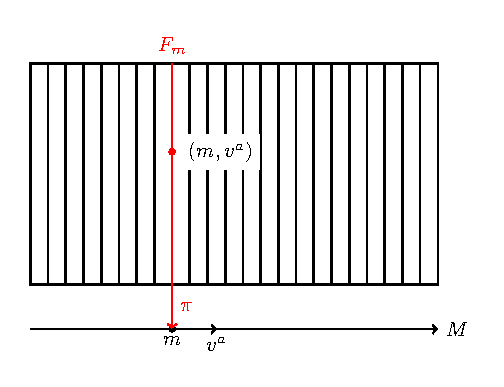
\includegraphics[width=0.5\textwidth]{../tikzpicture/tangentfiberbundles}
 \caption{切丛$TM$示意图}
 \label{fig:I-0-1}
 \end{figure}

 以$M$上方的竖直直线代表$F_m$,即一根\textbf{纤维(fiber)},$M$上的每一点都有一个 $F$,所有 $F$的集合记为$TM$,
 .取$m$的邻域 $O$,设$\{x^\mu\}$是 $M$的一个坐标系,则 $m$有 $n$个坐标, $v^a$也对应于
 n个实数 $v^\nu = v^a(dx^\nu)_a$,以 $(x^\mu,v^\nu)$ 作为点$(m,v^a)$的坐标变得TM的
 一个坐标系,可以把TM定义为一个2n维流形,称为流形的\textbf{切丛(tangent bundle)}.以上
 说明天然存在一个映射$\pi: TM \to M$,满足\[
 \pi((m,v^a)) = m
 .\]类似的可以定义\textbf{余切丛(cotangent bundle)} $T^* M$为 \[
 F^*_m \equiv \{(m,\omega_a) \mid\omega_a \in V^*_m\} 
 .\] 切丛和余切丛都是\textbf{纤维丛(fiber bundle)}的特例.

 本部分经常涉及丛流形P和底流形M,这里把$p \in P$的切空间记为$T_pP$,类似$m \in  M$的切空间记作 $T_mM$.
一个\textbf{纤维丛}由四元组 \((E, B, \pi, F)\) 构成,其中:
\begin{enumerate}
    \item \(E\) 称为\textbf{总空间}(total space),
    \item \(B\) 称为\textbf{底空间}(base space),
    \item \(F\) 称为\textbf{纤维}(fiber),
    \item \(\pi: E \to B\) 是一个连续满射,称为\textbf{投影映射}。
\end{enumerate}

满足以下条件:
\begin{enumerate}
    \item \textbf{局部平凡性}:对任意 \(x \in B\),存在开邻域 \(U \subseteq B\) 和同胚映射 \(\phi: \pi^{-1}(U) \to U \times F\),使得下图交换:
    \[
    \begin{array}{ccc}
        \pi^{-1}(U) & \xrightarrow{\phi} & U \times F \\
        \pi \downarrow & & \downarrow \mathrm{pr}_1 \\
        U & \xrightarrow{\mathrm{id}} & U
    \end{array}
    \]
    其中 \(\mathrm{pr}_1: U \times F \to U\) 是向第一个分量的投影。

    \item \textbf{转移函数的相容性}:若 \(U_i\) 和 \(U_j\) 是底空间 \(B\) 的两个相交开集,则存在转移函数(结构群 \(G\) 的作用):
    \[
        \phi_j \circ \phi_i^{-1}: (U_i \cap U_j) \times F \to (U_i \cap U_j) \times F,
    \]
    且对任意 \(x \in U_i \cap U_j\),映射 \(\phi_j \circ \phi_i^{-1}(x, \cdot): F \to F\) 属于结构群 \(G \subseteq \mathrm{Aut}(F)\)。
\end{enumerate}
以上定义是deepseek给出的,更为精确的定义可以参考其它文献.
 接下来就正式开始.
 \chapter{主纤维丛(Principal Fiber Bundles)}
 \section{定义和例子(definition and examples)}
 \begin{definition}
 {left action}{左作用} 
 李群G在流形K上的一个\textbf{左作用(left action)}是一个$C^\infty$映射$L:G \times K \to K$,满足:
 \begin{enumerate}
   \item $L_g: K \to K$是微分同胚$\forall  g \in  G$;
   \item $L_{gh} = L_g \circ L_h, \quad \forall g,h \in  G$.
 \end{enumerate}
\end{definition}
\begin{definition}
   {right action}{右作用} 
 李群G在流形K上的一个\textbf{右作用(right action)}是一个$C^\infty$映射$R:K \times G \to K$,满足:
 \begin{enumerate}
   \item $R_g: K \to K$是微分同胚$\forall  g \in  G$;
   \item $R_{gh} = R_h \circ R_g, \quad \forall g,h \in  G$.
 \end{enumerate}
\end{definition}
 \begin{note}
 考察$R_g(k), g\in G,k \in K$可以定义为$R_g(k) := kg \in K$,这是右作用;如果是左作用$L_g(k) := gk \in K$.
 有一点值得强调的是这里的$kg,gk$只是一种满足上面的定义,只要满足定义\ref{def:左作用},\ref{def:右作用}就可以,我们在后面\ref{thm:I-1-8}会有别的定义,如果不特殊声明,一般
 采用这里给出的定义.
 \end{note} 
 \begin{definition}
 {free}{自由的}
 右作用$R:P \times G \to P$称为\textbf{自由的(free)},若$g \neq e \Rightarrow pg \neq p \quad \forall p \in  P$;
 同理,左作用$R:G \times p \to P$称为\textbf{自由的(free)},若$g \neq e \Rightarrow gp \neq p \quad \forall p \in  P$.
 \end{definition}
 \begin{definition}
 {orbit}{轨道}
 子集$\{pg \mid g \in  G\} \subset P$ 称为右作用$R: P\times G\to P$过点$p \in P$的\textbf{轨道(orbit)};
 同理,子集$\{gp \mid g \in  G\} \subset P$ 称为左作用$R: G \times P\to P$过点$p \in P$的\textbf{轨道(orbit)}.
 \end{definition}
 \begin{figure}[htpb]
 \centering
 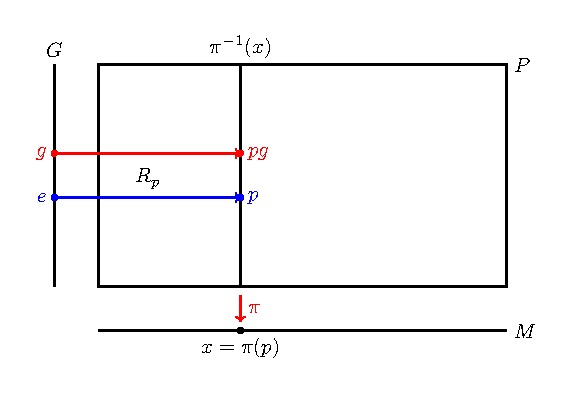
\includegraphics[width=0.5\textwidth]{../tikzpicture/principalfiberbundles}
 \caption{主纤维丛图示}
 \label{fig:I-1-1}
 \end{figure}
 \begin{definition}
 {principal fiber bundle}{主纤维丛}
 \textbf{主纤维丛(principak fiber bundle)}是由一个叫做\textbf{丛流形(bundle manifold)}的流形P、一个
 叫做\textbf{底流形(base manifold)}的流形M和一个叫做\textbf{结构群(structure group)}的李群组成,满足以下要求:
 \begin{enumerate}
   \item G在P上有自由右作用$R:P\times G \to P$;
   \item $\exists C^\infty$的、到上的投影映射$\pi: P \to M$,满足\[
       \pi^{-1}[\pi(p)] = \{pg  \mid g \in G\}, \quad \forall  p \in P;\text{见图}\ref{fig:I-1-1}
   .\] 
 \item  每一$x \in  M$有开邻域$U\subset M$及微分同胚$T_U: \pi^{-1}[U]\to U \times G$,且$T_U$取如下形式 \[
     T_u(p) = (\pi(p),S_U(p)),\quad \forall  p \in \pi^{-1}[U] 
   .\] 其中映射$S_U : \pi^{-1} [U] \to G$满足\[
  S_U(pg) = S_U(p)g,\quad \forall g \in G 
.\] 具体含义见图\ref{fig:I-1-2}
 \end{enumerate}
 \end{definition}
 \begin{note}
 原则上逆映射应该是一一到上的,可是第二条明显不是这样,在这里说的是集合之间的映射,$[\pi(p)]$应该理解为只有这一点的集合;[]代表集合的映射;
 为了便利起见,今后把主纤维丛简称为主丛,简记为$P(M,G)$或者 $P$.
 \end{note}
 由第一条知$R_p:G \to P,R_p(g) = R(p,g) = R_g(p)  \equiv pg$,结合第二条知道$pg \in \pi^{-1}[\pi(p)]$;结合图\ref{fig:I-1-1}给出具体的含义,随便给一个$p$点
 可以给出 $R_p$来,而 $R_p$作用于g,给出 $pg$和$p$同fiber,也就给出图中$pg$的位置,可见有\[
 R_p[G] = \pi^{-1}[\pi(p)] \Leftrightarrow R_p:G \to \pi^{-1}[\pi(p)] 
 .\] 事实上$R_p$是一个流形的嵌入映射,且为一个微分同胚映射,为什么是一个微分同胚映射,我们这里把其解释的更清楚一些,给定$p$后,与其同fiber的纤维便定了
 下来,满足条件2,即 \[
 g \in G \mapsto pg \in P 
 .\]如果g不同,则$pg$不同,反之亦然,再结合上右作用的要求 $C^\infty$,可见$R_p$是一个微分同胚映射;进一步要问,G的群结构是否也能被带到$\pi^{-1}[x]$上?是可以的,每一$p'\in \pi^{-1}[x]$对应于G的一个元素,即\[
 p' = R_p(g) = R_g(p) = pg 
 .\] 
 可以借用G的群乘法定义$\pi^{-1}[x]$的群乘法为\[
 (pg)\cdot (ph):= p(gh),\quad \forall pg , ph \in \pi^{-1}[x] 
 .\] 可以验证以上式定义的群乘法确实构成群,但是$\pi^{-1}[x]$不具有天生的群结构,群同构映射$R_p$是 $p$点依赖的.
 \begin{figure}[htpb]
 \centering
 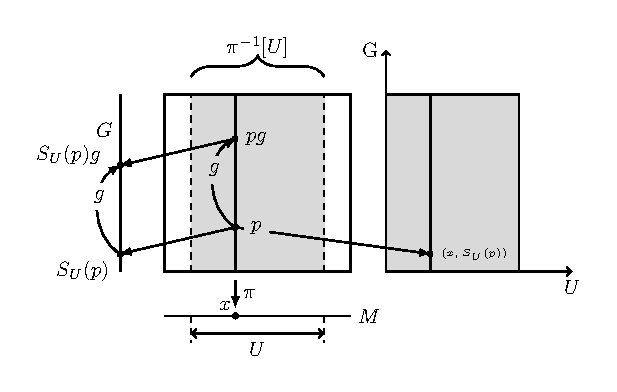
\includegraphics[width=0.6\textwidth]{../tikzpicture/S_U.pdf}
 \caption{条件3}
 \label{fig:I-1-2}
 \end{figure} 

 条件3很像是给主丛构建一个坐标系,借用卡式积的概念,如图\ref{fig:I-1-2},p点是主丛上的点,而其在底流形上的对应是固定的,由$\pi$映射到
 M上为x,抽象出来就是 $(x,\cdot)$,对于第二个就比较灵活,定义了 $S_U$映射,给出 $(x,S_U(p))$.如果x的U可以要求到$U = M$,则 $T_M : P \to M \times G$,也就意味着
 这时$P$和 $M\times G$微分同胚,此时的$P$是 \textbf{平凡(trivial) 主丛}.而当$U \neq M$,条件3要求$P$是局域平凡的,所以$T_U$是一个\textbf{局域平凡(local trivialization)}.
 由于$T_U$是微分同胚映射,不难给出 $\pi^{-1}[x]$与G之间的映射$S_U[\pi^{-1}[x]]$是微分同胚.因而可以在$\pi^{-1}[x]$上确定了一个特殊点$\breve{p}_U$,满足 $S_U(\breve{p}_U) = e \in G$, 结合主丛上定义的$R$,给出微分同胚映射 $R_{\breve{P}_U} : G \to \pi^{-1}[x]$,且$R_{\breve{P}_U}$与 $S_U:\pi^{-1}[x] \to G$互逆.
 \begin{theorem}
 {}{IB-1-1}
 $R_{\breve{P}_U}$ 与$S_U$互为逆映射.
 \end{theorem}
 \begin{proof}
 两个方向均是微分同胚映射,所以一一到上是绝对成立的,证明可逆只需要证明$R_{\breve{p}_U}\circ S_U = S_U\circ R_{\breve{p}_U} = e$
 \begin{enumerate}
 \item 证明$(R_{\breve{p}_U} \circ S_U) = e$
   \begin{align*}
 (R_{\breve{p}_U} \circ S_U)p = R_{\breve{p}_U}S_U(p) = R_{S_U(p)}\breve{p}_U  = \breve{p}_U S_U(p)  
 \end{align*}
 由于$p,\breve{p}_U \in  \pi^{-1}[x]$,不难知道存在g满足$p = \breve{p}_U g$代入上式中有 \[
 (R_{\breve{p}_U} \circ S_U)p = \breve{p}_U S_U(\breve{p}_U g) = \breve{p}_U S_U(\breve{p}_U)g = \breve{p}_Ueg = p
 .\] 
 所以等式成立.
 \item 证明$(S_U \circ R_{\breve{p_U}}) = e$
 \begin{align*}
   (S_U \circ R_{\breve{p_U}}) g =S_U(R_{\breve{p}_U}(g)) = S_U(\breve{p}_U g) = S_U(\breve{p}_U)g = eg = g 
 .\end{align*}
 等式成立.
 \end{enumerate}
 \end{proof}
 \begin{example}
 \label{ex:I-1-1}
 对任给的李群G和流形M总可以按如下三步构造一个主丛:
 \begin{enumerate}
   \item 选择 $P \equiv M \times G$ 为丛流形,则P的任一点都可以表为$p = (x,g),x \in M, g \in G$ 
   \item 定义自由右作用$R: P \times G \to  P$为\[
       R_h(x,g) := (x,gh),\text{即}(x,g)h = (x,gh),\quad \forall x \in  M , h,g \in G  
   .\] 
 \item 定义投影映射为\[
\pi(x,g):= x, \quad x\in M,g\in G 
 .\] 
 \end{enumerate}
 以上构造的主丛是平凡的
 \end{example}

 设 $P(M,G)$是主丛, $T_U : \pi^{-1} [U] \to  U \times G$ 和$T_V: \pi^{-1}[V] \to V \times G$是两个局域平凡的
 ,且$U \cap V \ne \varnothing$,每一个$p \in  \pi^{-1}[U\cap V]$在G上有两个像点,为
 $g_U = S_U(p), g_V = S_V(p)$故有$T_U(p) = (x,g_U),  T_V = (x,g_V)$
 很明显$T_U \cup T_V \supset P$,原因很简单,$\pi^{-1}[U \cap V]$内的每一个元素对应于两个点(或更多,如果交的集合增加的话),如果把这两个像点认为是同一个点,那么
 $P = T_U \cup T_V = P$,也就天然的要求\[
 g_U = g_U g_V^{-1}g_V = S_U(p)S_V(p)^{-1}g_V
 .\] 由此可以给出如下定义
 \begin{definition}
 {transition function}{转换函数}
 设$T_U : \pi^{-1}[U] \to U\times G$和$T_V : \pi^{-1} [V] \to V\times G$是主丛$P(M,G)$的两个局域平凡, $U \cup V \neq \varnothing $.映射$g_{UV} : U\cap V \to G$称为$T_U$到 $T_V$ 的\textbf{转换函数(transition function)},若
 \[
   g_{UV}(x) = S_U(p)S_V(p)^{-1},\quad \forall x \in U \cap V,\quad \pi(p) = x
 .\]
 \end{definition}
 有了上面定义,难免会遇到这样的一个问题$p'$和 $p$是有可能对应同一个x(二者同fiber就行,同时意味着$p',p$中间满足 $p' = pg$),但是两者生成的 $g_{UV}$是否还一致,我们来看
 \begin{align*}
 S_U(p')S_V(p')^{-1} = S_U(pg)S_V(pg)^{-1} = S_U(p)g(S_V(p)g)^{-1} = S_U(p)gg^{-1}S_V(p)^{-1} = S_U(p)S_V(p)^{-1}
 .\end{align*}
 由此说明无论是哪个$p$,只要映射到同一个 $x$,之间的转换函数就是一样的.

 \begin{theorem}
 {}{I-1-1}
 $g_{UV}$满足如下性质
  \begin{enumerate}
    \item $g_{U U} = e, \quad \forall U\cap V ;$
    \item $g_{VU}(x) = g_{UV}(x)^{-1} , \quad \forall x \in U\cap V;$
    \item $g_{UV}(x) g_{VW}(x) g_{WU}(x) = e,\quad \forall x \in U\cap V\cap W$
 \end{enumerate}
 \end{theorem}
 证明上面等式比较简单,代入定义\ref{def:转换函数}便可以轻松看出.上文提出,在$U\cap V \neq \varnothing$中,每一个$p$可以经过
$T_U,T_V \cdots$映射到不同的的点,为了保证P不变,我们引入了转换函数,更具体而言,就是定义了一个等价关系
\begin{equation}
  x = x' , g = g_{UV}(x)g' \quad (x,g) \in  U\times G , (x',g') \in  V\times G
  \label{eq:I-1-1} 
\end{equation}
此时认为$(x,g)$等价于 $(x',g')$记作 $(x,g) \sim (x',g')$,数学上的等价关系必须具备如下性质.
\begin{enumerate}
  \item \textbf{反身性}: 一个元素等价与自身,即,$(x,g) \sim (x,g)$;
  \item \textbf{对称性}: a等价于b,则b等价于a,即$(x,g) \sim (x',g') \Leftrightarrow (x',g') \sim (x,g)$;
  \item \textbf{传递性}: a等价于b,b等价于c,则a等价于c,即$(x,g)\sim (x',g'),(x',g') \sim (x'',g'') \Rightarrow (x,g) \sim (x'',g'')$.
\end{enumerate}
接下来让我们验证我们定义的式子\ref{eq:I-1-1}满足以上三个性质
\begin{enumerate}
  \item 反身性:由式\ref{eq:I-1-1}知 \[
      x = x,g = g_{U U}g = g
  .\] 可知反身性成立.
\item 对称性:已知 $(x,g) \sim (x',g')$,即\[
    x = x' ,g = g_{UV} g'
.\]很轻松得到$x' = x$,对于另一个式子我么有
\begin{align*}
  g' = g_{UV}(x)^{-1}g = g_{VU}(x)g
\end{align*}
根据式子\ref{eq:I-1-1}知道$(x',g') \sim (x,g)$,对于反向的过程与之十分相似,这里不证.
 \item 传递性:已知$(x,g)\sim (x',g'),(x',g') \sim (x'',g'')$,即\[
   x = x' \quad g = g_{UV}(x)g'\quad x' = x'' \quad g ' = g_{VW}g''
 .\]
 不难给出$x = x''$,对于另一个式子有 \[
 g = g_{UV}g_{VW} g= g_{UW} 
 .\] 则$(x,g) \sim (x'',g'')$
\end{enumerate}
\begin{note}
 注意:U对应于$(x,g)$ ,V对应于$(x',g')$,W对应于 $(x'',g'')$.
\end{note}
\begin{theorem}
  {}{I-1-2} 
  设$g_{UV}$是从局域平凡$T_U$到 $T_V$的转换函数, $x\in  U \cap V$,以$\breve{p}_U$和$\breve{p}_V$分别代表由 $T_U$和$T_V$在 $\pi^{-1}[x]$上确定的特殊点,定义为
  \[
    S_U(\breve{p}_U) = S_V(\breve{p}_V) = e \in  G
  .\]则
  \[
    \breve{p}_V = \breve{p}_U g_{UV}(x)
  .\] 
\end{theorem}
\begin{proof}
  $\breve{p}_U,\breve{p}_V \in \pi^{-1}[x]$保证$\exists g \in G$使\[
    \breve{p}_V = \breve{p}_U g
  .\]  
  前文说明只要$\pi^{-1}[x]$相同,$g_{UV}$的选择与 $p$无关,不妨选择 $\breve{p}_V$
  \begin{equation*}
    g_{UV}(x) = S_U(\breve{p}_V)S_V(\breve{p}_V)^{-1} = S_U(\breve{p}_V) = S_U(\breve{p}_Ug) = eg = g
  \end{equation*}
  故有\[
    \breve{p}_V = \breve{p}_U g_{UV}(x)
  .\] 
\end{proof}
\begin{definition}
  {local (cross) section}{局域截面}
  设$P(M,G)$是主丛, $U$是 $M$的开子集. $C^\infty$映射 $\sigma: U \to P$称为一个\textbf{局域截面(local (cross)section)}若\[
  \pi(\sigma(x)) = x, \quad \forall x \in U
  .\] 
\end{definition}
\begin{theorem}
  {}{I-1-3}
  局域截面和局域平凡之间存在一一对应关系.
\end{theorem}
\begin{proof}
  定理是存在性,证明二者是可以通过构造的方法.
  \begin{enumerate}
    \item 局域平凡可以给出一个局域截面\\
  选定$T_U:\pi^{-1}[U]\to U\times G$后每一个$x\in U$会有一个特殊点$\breve{p}_U$,就是上文中给出如下等式的那个点
  \[
  S_U(\breve{p}_U) = e \in G
  .\] 
  每有一个$x$便有一个 $\breve{p}_U$,即$\breve{p}_U(x)$,定义\[
 \sigma(x) := \breve{p}_U(x) 
  .\]
  我们给出了一个映射$U\to P$,接下来需要证明其是否是$C^\infty$的,首先$T_U(x,S_U(\breve{p}_U(x))$ 是$C^\infty$的,又因为\[
 T_U(x,S_U(\breve{p}_U(x))) = T_U(x,e) 
  .\]
  不难看出$U$和$\{\breve{p}_U[U]\}$ 是微分同胚的.
  \begin{note}
    这里hand-waving一下,上面的思路是底流形M是连续的(即$M$与 $\mathbb{R}^n$微分同胚),而选定$\breve{p}_U$ 的集合作为这个截面的映射,是因为这样相当于2维坐标系中,y是常数,x变化引出的曲线与x轴内
    对应的集合微分同胚,在这里就是$U$和$\{\breve{p}_U[U]\}$微分同胚.
  \end{note}
\item 给定局域截面可以构造一个对应的局域平凡.
  给定$\sigma: U \to P$后,令$\sigma(x)$为作为特殊点 $\breve{p}_U$,对于和$\sigma(x)$共纤维的点p有等式 $p = \sigma(x)g$,对于$\forall p \in \pi^{-1}[U]$定义\[
 T_U(p) := (x,g) 
 .\] 
 这要验证上式满足定义\ref{def:主纤维丛}第三点中$S_U$的性质,而这个性质就是说在$\pi^{-1}[x]$上群元之间的关系和G的对应群元关系相同,我们这里那$\pi^{-1}[x]$的群元关系定义为$S_U$,自然满足,我们
 就构造了一个局域平凡的映射,并且特殊点为$\sigma(x)$.
  \end{enumerate}
  这样我们就建立起来了局域平凡和局域截面的一一对于关系.
\end{proof}
我们构造出$\sigma(x) \sim \breve{p}(x)$,故$\sigma(x)$满足如下等式 
 \begin{equation}
 \sigma_V(x) = \sigma_U(x)g_{UV}(x)\quad \forall x\in U\cap V 
 \label{eq:I-1-2} 
 \end{equation}
 \begin{definition}
 {global section}{整体截面}
 局部截面$\sigma:U \to P$称为\textbf{整体截面(global section)},若$U = M$.
 \end{definition}

 对应于平凡主丛,会有整体截面的概念,上面定义也满足平凡主丛的要求,不过由于局部平凡的主丛更有用,所以整体截面很少见到.

 \begin{example}
 \label{ex:I-1-2}
 设$M = S^1,G = Z_2$, $S^1$是一维圆周, $Z_2 = \{e,h\}$是0维李群,其中$eh =he =h, hh = e$,按照例\ref{ex:I-1-1}可以构造一个平凡主丛$P = S^1 \times Z_2$,
 不难看出$P$是两个不连通的圆周的并,对主丛加以修改得到非平凡主丛,见例\ref{ex:I-1-3}
 \end{example}
 \begin{example}
 \label{ex:I-1-3}
 令$P = S^1,G = Z_2$, $S^1,Z_2$和例\ref{ex:I-1-2}一致.需要定义右作用$R:P\times G \to P$,即$R: S^1 \times Z_2 \to S^1$,按照如下定义
 \begin{align*}
   R_e(p_\theta)&:= p_\theta\\
   R_h(p_\theta)&:= p_{\theta+\pi}
 .\end{align*}
 $\theta$是圆周上的角度坐标.
 如图\ref{fig:I-1-3}所示,根据定义的右作用可以给出虚线两个端点同fiber,把下半圆投影到下方直线再加上端点认同下方直线就是底流形$M$,由于对径认同$M$和 $S^1$有相同的拓扑结构,也就是 $\{a_1,a_2\}$投影到 $a$点,其它类似.
 此时$P \neq M\times G$,原因是 $M \times G = S^1 \times G$是两个圆周,而 $P$是一个自然就不是平凡主丛.
 更形象的图见书p1089,图I-7.
 \begin{figure}[htpb]
   \centering
   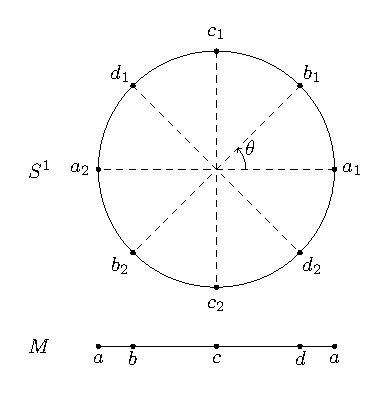
\includegraphics[width=0.5\textwidth]{../tikzpicture/exI13.pdf}
   \caption{例3}
   \label{fig:I-1-3}
 \end{figure}
 \end{example}
 \begin{example}
   \label{ex:I-1-4}
   设$M$是 $n$维流形,以 $T_xM$代表 $x\in M$的切空间,令\[
 P \equiv \{(x,e_\mu)| x \in  M, \{e_\mu\} \text{是}T_xM\text{的一个基底}\}
   .\]

   首先看$P$是否是一个流形;
   设$(O,\psi)$是M的一个坐标系,坐标为$\{x^\mu\}$,则每个 $e_\mu$可以使用坐标基底展开 \[
  e_\mu = e^{\nu}{}_{\mu} \frac{\partial }{\partial x^\nu}  
   .\] 
   则$(x,e_\mu)$可以用一组实数 $(x^\sigma,e^{\nu}{}_{\mu})$ 来刻画,共计$n + n^2$个,也就是说$P$上存在坐标
   $(x^\sigma,e^{\nu}{}_{\mu}) \in  R^{n + n^2}$,流形的定义有两点,1任意开覆盖子集同胚于用$\mathbb{R}^n$刻画的开子集;2
   重叠的区域诱导出的多个 $\mathbb{R}^n$之间的映射是 $C^\infty$,对于M本身的要求只有第一点,
   这里已经满足了.故$P$是一个流形.

   根据主丛的要求,可以选$GL(n)$为结构群$G$,通过以下三步构造一个主丛
   \begin{enumerate}
     \item 定义矩阵群$GL(n)$在P上的自由右作用 $R:P \times GL(n) \to P$为\[
         R_g(x,e_\mu) := (x,e_\nu g^{\nu}{}_{\mu}), \quad \forall g \in GL(n) 
     .\]
     GL(n)是可逆映射不会改变基矢之间的线性独立性,因此会变换到新的基矢量;
   \item 定义投影映射$\pi : P \to M$为$\pi(x,e_\mu) := x, \quad \forall (x,e_\mu) \in  P$ ;
   \item $\forall x \in M$,总有坐标系$\{x^\mu\}$其坐标域U含x.定义局域平凡$T_U : \pi^{-1} [U] \to  U \times G$为 \[
      T_U(x,e_\mu):= (x,h)
       .\]
     其中$h \equiv S_U((x,e_\mu))$满足如下等式 \[
    \frac{\partial   }{\partial x^\nu} \mid _x h^{\nu}{}_{\mu} = e_\mu \Leftrightarrow S_U((x,e_\mu)) = e_\nu h^{\nu}{}_{\mu}
     .\]
     接下来需要验证$h$ 满足如下等式\[
    S_U((x,e_\mu)g ) = S_U((x,e_\mu))g 
     .\] 
     用第二个式子更好给出
     \begin{align*}
      S_U((x,e_\mu)g) = S_U((x,e_\mu g)) = e_\nu h^{\nu}{}_{\mu}g = S_U((x,e_\mu))g
     .\end{align*}
     \begin{note}
       事实上$g$也应该写上指标,不过这里足够清楚,就没有遵守指标的一个平衡.
     \end{note}
   \end{enumerate}
   由于$\det(g^{\mu}{}_{\nu}) \neq = 0$ 且有限维的线性映射总是光滑的,不难给出$T_U$是微分同胚的.
 \end{example}

 由于基底又名标架,所以由以上构造出的主丛$P(M,GL(n))$称为\textbf{标价丛(frame bundle)}
 \begin{example}
 \label{ex:I-1-5}
 若在$M$上定义了度规场,对于标架而言便可以讨论正交归一性.以洛伦兹时空为例 \[
   P \equiv \{x, \hat{e}_\mu  \mid x \in M\} \hat{e}_\mu\text{代表}T_xM\text{上的正交归一基底} 
 .\] 
 选择$O(1,3)$为结构群的话,按照例\ref{ex:I-1-4}定义给出的主丛称为\textbf{正交归一标价丛(orthogonal frame bundle)}.

 \end{example}
 \section{主丛上的基本矢量场(Fundmental Vector Feilds)}
 主丛P上的每点p可以定义切空间$T_pP$,同样的对于过$p$点的纤维$\pi^{-1}[\pi(p)]$可以给出其切矢$X$,它们之间的关系是
 \[
   X \in T_p\pi^{-1}[\pi(p)] \subset T_pP
 .\] 
 具体理解为$X$切于过 $p$点的躺在 $\pi^{-1}[\pi(p)]$上的一条曲线,$\pi$把这条曲线映射到一点 $\pi(p)$,
 我们定义的推前映射(切映射) $\pi_*$可以给出切矢量在底流形的像,由于底流形上只有一点,故而有 \[
   \pi_*(X) = 0
 .\] 
 不妨令$V_p = T_p\pi^{-1}[\pi(p)]$,则可以给出$V_p$的定义式 \[
   V_p := \{X \in T_pP  \mid  \pi_*(X) = 0\}
 .\] 
 把满足$\pi_*(X) = 0$的 $X$称为\textbf{竖直矢量},把 $V_p$称为\textbf{竖直子空间(vertical subspace)}.
 \begin{note}
   根据图\ref{fig:I-1-1}容易把X理解为垂直于$M$的矢量,这是片面的,如果李群 $G$是多维度的, $\pi$依旧会将其
   映射到一个点,但是此时的 $M$却不一定垂直于 $M$.
 \end{note}
 \begin{theorem}
   {}{I-1-4}
   设$P(M,G)$是主丛, $V_p$是点 $p \in  P$的切空间$T_pP$的竖直子空间, $\mathscr{G}$是G的李代数,则$V_p$与 $\mathscr{G}$作为矢量空间
   有自然的同构映射.
 \end{theorem}
 \begin{proof}
   右作用$R:P \times G \to P$对每一个p给出一个微分同胚映射$G \to \pi^{-1}[\pi(p)]$,且$R_p(e) = p$,所以
   $R_p$在恒等元 $e \in G$给出推前映射$R_{p*} :T_eG \to T_p \pi^{-1}[\pi(p)]$,而$\mathscr{G}$同构于
   $T_eG$, $V_p = T_p\pi^{-1}[\pi(P)]$故$R_{p*} : \mathscr{G}\to V_p$,微分同胚映射诱导出来的切映射自然
   是一一对应的,不难给出两个矢量空间同构.
 \end{proof}
 \begin{definition}
   {Fundmental Vector Field}{基本矢量场}
   给定$A\in \mathscr{G}$后,每点$p \in P$可以给出一个竖直矢量$A^*_p$ \[
     A^*_p := R_{p*} A , \forall p \in P
   .\] 
   因而每一$A\in \mathscr{G}$ 在$P$上胜出一个竖直矢量场 $A^*$,称为由 $A$诱导的\textbf{基本矢量场(fundmental vector field)}
 \end{definition}
 \begin{theorem}
   {}{I-1-5}
   设$T_U$是局域平凡, $x\in U$,则微分同胚$S_U:\pi^{-1}[x] \to G$的推前映射$S_{U*}$把 $\pi^{-1}[x]$上的基本矢量场$A^*$映为 $G$上由 $A \in \mathscr{G}$生成的左不变矢量场$\overline{A}$,即
   \[
     S_{U*}A^* = \overline{A}
   .\] 
 \end{theorem}
 \begin{proof}
   $\forall p \in \pi^{-1}[x]$,令\[
   g \equiv S_U(p) \in G
   .\] 
   只需要验证$S_{U*}$把 $p$点的基本矢量场映射为左不变矢量场在$g$点的值即 \[
     S_{U*}A^*_p = \overline{A}_g
   .\] 
   首先$\overline{A}_g = L_{g*}A$,$L_g:G \to G$是由$g \in G$生成的左平移映射,
   对于任意 $g' \in G$,有 \[
     R_{pg}g' = R_{g'}(pg) = pgg' = R_{gg'}(p) = R_p(gg') = R_p(L_g(g')) = R_p \circ L_g (g')
   .\] 即$R_{pg} = R_p \circ L_g$;另外由$g = S_U(p)$不难给出 \[
   p = S_U^{-1}(g) = R_{\breve{p}_U}(g) = \breve{p}_Ug
 .\]引用了定理\ref{thm:IB-1-1}.\\
 故
 \begin{align*}
   S_{U*} A^*_p &= S_{U*} R_{p*}A\qquad \text{定义}\ref{def:基本矢量场}\\
                &= S_{U*} R_{\breve{p}_Ug*}A\\
                &= S_{U*}(R_{\breve{p}_U} \circ L_g)_*A\\
                &= (S_U\circ R_{\breve{p}_U})_* L_{g*}A\\
                &=(e)_* L_{g*}A\\
                &= (L_{e}\circ L_g)_*A\\
                &= L_{g*}A = \overline{A}_g
 .\end{align*}
 \end{proof}

 矢量$A \in T_eG$作为生成元,可以在$G$上生成一个单参子群 $\exp(tA)\in G, t\in \mathbb{R},A \in \mathscr{G} = T_eG$,
 结合 $ p \in P$可以给出$\pi^{-1}[\pi(p)]$内的一条曲线,其在$p$点的切矢是 $A^*_p$,表述为如下定理.
  \begin{theorem}
    {}{IB-1-2}
    $A^*_p = \left.\frac{d}{dt}\right|_{t=0} [p(\exp(tA)]$
 \end{theorem}
 \begin{proof}
 \[
   A^*_p = R_{p*}A = R_{p*}\left[ \left.\frac{d}{dt}\right|_{t=0} \exp(tA) \right] = \left.\frac{d}{dt}\right|_{t=0}[R_p \exp(tA)] = \left.\frac{d}{dt}\right|_{t=0}[p \exp(tA)]
     .\]
      \begin{note}
      这里使用的基本原理是像的切矢等于切矢的像. 
     \end{note}
 \end{proof}
 \begin{theorem}
   {}{I-1-6}设$P(M,G)$是主丛, $A\in T_eG, t\in \mathbb{R}$,定义$\phi_t : P \to P$为\[
  \phi_t(p) := p \exp(tA), \quad \forall p \in P 
.\]则$\{\phi_t \mid t \in \mathbb{R}\}$是由矢量场$A^*$产生的单参微分同胚群.
 \end{theorem}
 \begin{proof}
   $\forall p \in P,\phi_t(p) = p\exp(tA) = R_{\exp(tA)}(p)$,在定义\ref{def:主纤维丛}下面我们说明了$R_g$是微分同胚映射,对应到这里就是 $\phi_t$是微分同胚映射.
   根据单参子群的定义要求$\phi_t$为 $C^\infty$曲线且满足$\phi_{t+s} = \phi_t\circ \phi_s$,我们逐步来看,首先不妨令\[
  \gamma(tA) = \exp(tA)
   .\] 在第四章中曾说明$\gamma(t)$是单参子群,也就是说存在两次映射 \[
  t \mapsto \gamma(tA) \mapsto \phi_t(p) 
   .\] 这两次均是$C^\infty$的,所以对于第一个条件满足,我们来看第二个
   \[
     (\phi_t\circ \phi_s)(p)=\phi_t(p) \circ \phi_s(p) = (p(\exp(tA)))\cdot(p(\exp(sA))) = p(\exp(tA)\exp(sA)) = p (\exp((t+s)A)) = \phi_{t+s}(p)
   .\] 
   \begin{note}
     注意这里定义的群乘法和G上的不同,这里定义的群乘法在定义\ref{def:主纤维丛}下方;对于第一个等号而言我们给出\[
     (\phi_t\circ \phi_s)(p)= (\phi_t)(\phi_s(p)) = \phi_t(p\exp(tA)) = p(\exp(tA)\exp(sA))
     .\] 根据定义的群乘法给出了第一个等号(这个等号描述的是同一个东西本该相等,这里只是验证一下),这也从侧面说明这样群乘法定义的合理性.
   \end{note}
 目前为止,我们说明了$\phi_t$是单参子群,又因为是微分同胚映射,故$\phi_t$是单参微分同胚群(定义见书P46),接下来只需要证明其是由 $A^*$产生的即可,也就是说证明
 $p(\exp(tA)$是 $A^*$的积分曲线,即证明 $\left.\frac{d}{dt}\right|_{t=s}p\exp(tA) = A^*_{\phi_s(p)}$
  \begin{align*}
    A^*_{\phi_s(p)} &=  \left.\frac{d}{dt}\right|_{t=0} [\phi_s(p)(\exp(tA)] \quad \text{定理}\ref{thm:IB-1-2}\\ 
                    &= \left.\frac{d}{dt}\right|_{t=0}[p\exp(sA) \exp(tA)]\\
                    &=\left.\frac{d}{dt}\right|_{t=0}[p\exp(t+s)A]\quad \text{令}t' = t+s\\
                    &= \left.\frac{d}{dt}\right|_{t'=s} p \exp(t'A) \quad \text{令} t = t'\\
                    &=\left.\frac{d}{dt}\right|_{t=s}p\exp(tA)
 \end{align*}
 至此证明结束.
 \end{proof}
 \begin{theorem}
   {}{I-1-7}
   竖直矢量场$A^*$服从如下公式 \[
     R_{g_*}A^*_p = (\mathscr{A}\!d_{g^{-1}}A)^*_{pg}, \quad \forall p \in P, g\in G, A \in \mathscr{G} 
   .\] 
 \end{theorem}
 \begin{proof}
  \begin{align*}
    R_{g_*}A^*_p &= R_{g*}\left.\frac{d}{dt}\right|_{t=0} [p(\exp(tA)] \quad\text{定理} \ref{thm:IB-1-2}\\
                 &= \left.\frac{d}{dt}\right|_{t=0} R_g [p(\exp(tA)] = \left.\frac{d}{dt}\right|_{t=0} p(\exp(tA)g\\
                 &= \left.\frac{d}{dt}\right|_{t=0} pgg^{-1}(\exp(tA))g \\
                 &= \left.\frac{d}{dt}\right|_{t=0}R_{pg}(g^{-1}(\exp(tA))g)\quad \text{注意分清P的元素和G的元素}\\
                 &= R_{pg*}\left.\frac{d}{dt}\right|_{t=0}(I_{g^{-1}}(\exp(tA))) \quad \text{利用了伴随表示的定义} \\
                 &= R_{pg*}(I_{g^{-1}*}A) = R_{pg*}(\mathscr{A}\!d_{g^{-1}*}A)\quad \text{见第8章定义}\\
                 &=(\mathscr{A}\!d_{g^{-1}}A)^*_{pg}
  .\end{align*} 
 \end{proof}
 \begin{note}
   该定理表述了由$A$生成的竖直矢量场在 $p$点的值经过 $g$的右作用诱导出的推前映射所得的像等于 $A$经过$g^{-1}$伴随表示 的切映射生成的矢量场在$pg$的值.
 \end{note}

 \begin{theorem}
 {}{I-1-8}
 设$[A,B] \in  \mathscr{G}$是$A,B \in \mathscr{G}$的李括号,$[A^*,B^*]$是矢量场$A^{*},B^{*}$ 的对易子,则$P$上有矢量场等式 \[
   [A^*,B^*] = [A,B]^* 
 .\] 
 \end{theorem}
 \begin{proof}
这个定理所要表达的含义就是 

借助右作用可以定义李变换群(G对P的左作用)为\[
  \sigma(g,p) := R_{g^{-1}}(p)
.\]
不难验证$\sigma_{gh}(p) = R_{(gh)^{-1}}(p) = ph^{-1}g^{-1} = R_{g^{-1}} \circ R_{h^{-1}}(p)$满足定义\ref{def:左作用}的要求2,第一点由
右作用自动满足.

对于李变换群上的每一个单参微分同胚群存在映射$\chi:\mathscr{G} \to \mathscr{K}$与之对应的$C^\infty$矢量场$\overline{\xi}$ \[
  \overline{\xi} = \left. \frac{d}{dt} \right|_{t = 0}\sigma_p(\exp(tA)) = \left. \frac{d}{dt} \right|_{t = 0} R_p(\exp(-tA)) 
      = R_{p*}(-A) = -A^*_p
.\] 
故$\chi(A) = -A^*$,根据第七章内容有李代数同构 $\psi:\mathscr{G} \to \mathscr{K}$满足$\psi(A) = A^*$保李括号,于是 \[
  [A^*,B^*] = [\psi(A),\psi(B)] = \psi([A,B]) = [A,B]^*
.\] 
 \end{proof}
\chapter{主丛上的联络(Connection In a Principal Fiber Bundle)}
 在主丛$P$上定义一个称为联络的附加结构,后便可讨论水平子空间,这里不太严谨的说明一下,正如图\ref{fig:I-1-2}右面
 显示的那样,竖直子空间是G方向的矢量空间,水平子空间是U方向的矢量空间.
 \section{主丛联络的三个等价定义(Three Equivalent Definitions of Connection)}
 介绍定义之间补充关于直和的概念.
 \begin{definition}
   {direct sum}{直和}
   矢量空间$V$称为其子空间 $V^1$和 $V^2$的\textbf{直和(direct sum)},记\[
   V = V_1 \oplus V_2
   .\] 
   若$v \in V$有唯一的$v_1 \in V_1$和$v_2 \in V_2$,使 \[
   v = v_1 + v_2
   .\] 
 \end{definition}
 不难给出
 \begin{enumerate}
   \item $\dim(V_1 \oplus V_2) = \dim V_1 + \dim V_2$;
   \item  $V_1 \cap V_2 = \{0\} \subset V$
 \end{enumerate}
\begin{proof}
  \begin{enumerate}
    \item 对于$\forall v \in V$,有\[
        \dim(v) = \dim(v_1 + v_2) \quad \exists v_1 \in V_1,V_2 \in V
        .\]  由于$v_1$, $v_2$线性无关,则 \[\dim(v_1 + v_2) = \dim(v_1) + \dim(v_2).\]
        对$\forall v \in  V$成立,即\[
          \dim{V} = \dim{V_1} + \dim{V_2}
        .\] 
      \item 首先$V_1 \subset V,V_2\subset V$,对于$v \in V_1 or v\in V_2$,要想满足式子$v = v_1 + v_2$,则
        三者都有零元,假设$V_1\cap V_2$有除去零元的元素$v_{1a},a = 1,2$代表属于不同的空间.
        假设 $v \in V$,有\[
          v = v_{11} + v_{2} = v_{12} + v_{2} 
        .\] 
        可以看出$\exists $情况$v_{11} \neq 0$,  $v_2 \neq v_{12} + v_2$,我们找到了第二种组合,与定义\ref{def:直和} 要求不符合,故没有除了零元外的集合.
  \end{enumerate}
\end{proof}
\begin{definition}
  {Connection(1)}{联络-1}
主丛$P(M,G)$上的一个\textbf{联络(connection)}是对每点$p \in  P$指定一个\textbf{水平子空间(horizontal subspace)}$H_p \subset T_pP$,满足
\begin{enumerate}
  \item $T_pP = V_p \oplus H_p, \quad \forall  p \in P$;
  \item $R_{g*}[H_p] = H_{pg},\quad \forall p\in P, g \in G $;
  \item $H_p$光滑地依赖于 $p$.
\end{enumerate}
\end{definition}
  条件1不难理解,条件2要求$T_pP$的 $H_p$在 $R_{g*}$作用下的像等于 $T_{pg}P$的水平子空间,这个定义非常自然;条件3的准确含义是:每一$p \in P$有邻域$N$,其上存在 $n = \dim M$个光滑矢量场,它们在任一 $q \in N$的值可以当作
  $H_q$的基底.

  $\pi: P \to M$在点$p \in P$的推前映射$\pi_* : T_pP \to T_xM$把$\pi_*$的定义域限制到 $H_p$上,我们自然希望 $\pi_*: H_p \to T_xM$是一个同构映射,下面来证明:
  \begin{align*}
    \dim H_p &= \dim T_pP - \dim V_p = \dim P - \dim \mathscr{G} \\&=  \dim(M \times G) - \dim{G} = \dim{M} + \dim{G} -\dim G = \dim M = \dim T_xM
  \end{align*}
  既然$H_p$和 $T_xM$维度相同,在这个前提下我们只需要证明一一性或到上性两者之一,这里证明一一性.
   \begin{note}
   如果映射前后的矢量空间同维度,如果一一性成立,也就是说$H_p$势必会在 $T_xM$上的不同的像上, 我们讨论的均为线性映射,也就是说不改变线性独立性,则映射过去的像可生成矢量空间$T_xM$即是到上的;
   反过来,如果映射到上性成立,也就是说, 每一个$T_xM$都会有逆像,同样的由于线性独立性,加上同维的话,每个逆像只会有一个,也就是一一性成立.
  \end{note}
  设存在$X,X' \in H_p$使得$\pi_* X = \pi_* X'$,则 $\pi_*(X - X') = 0$,根据竖直子空间定义给出$X - X' \in V_p$,又因为$X,X' \in H_p$,所以$X - X' \in  H_p$,再结合上$V_p \cap H_p = \{0\}$,故
  \[
 X - X' = 0 
  .\] 
  所以一一性成立,每个$T_xM$只会对应于一个逆像,最后给出 $H_p$同构于 $T_xM$.

  在阐述第二个定义之前,还需要补充一些数学知识,假设我们有一个流形$M$其上存在映射 $f:M\to \mathbb{R}$,此时$f$是 $M$上的0形式场(标量场函数)
以$\Lambda_M(0)$代表光滑的0形式场,如果 $f$是光滑的,则有 $f \in \Lambda_M(0)$
\begin{note}
  如果$f:M \to \mathbb{R} or \mathbb{C}$,那么$f \in \Lambda_M(0,\mathbb{R} or \mathbb{C})$,即实数取值或复数取值的0形式场.
\end{note}
进一步可以推广到矢量空间的0形式场,如果$f^1 ,\cdots ,f^R \in \Lambda_M(0,\mathbb{R} or \mathbb{C})$,$e_r \in$矢量空间$\mathscr{V}$,令\[
f \equiv e_1f^1 +\cdots + e_R f^R = e_r f^r
.\] 
则有\[f(x) = e_rf^r(x) \in \mathscr{V},x\in M\]
这样我们给出了$f \in \Lambda_M(0,\mathscr{V})$.

接下来我们给出$l$形式场,我们假定$\varphi^1,\cdots ,\varphi^R \in \Lambda_M(l, \mathbb{R} or \mathbb{C})$,再配上矢量空间基矢,有\[
\varphi \equiv e_r\varphi^r \in\Lambda_M(l,\mathscr{V}) 
.\] 
则对于$v_1,\cdots,v_l$是 $M$上x点的矢量 \[
\left.\varphi\right|_x(v_1,\cdots,v_l) := e_r\varphi^r|_x(v_1,\cdots , v_l) \in \mathscr{V} 
.\] 
我们接下来给出微分形式\[
d\varphi = e_r d\varphi^r \in\Lambda_M(l+1,\mathscr{V}) 
.\] 
\begin{definition}
  {Connection(2)}{联络-2}
  主丛$P(M,G)$上的\textbf{联络}是 $P$上的一个 $C^\infty$的$\mathscr{G}$值$1$(一)形式场$\bm{\tilde{\omega}} $,满足:
 \begin{enumerate}
   \item $ \bm{\tilde{\omega}}(A^*_p) = A, \quad \forall A \in \mathscr{G},p \in P $ ;
   \item $\bm{\tilde{\omega}}_{pg}(R_{g*}X) = \mathscr{A}\!d_{g^{-1}} \bm{\tilde{\omega}}_p(X), \quad \forall p \in P, g \in G, X \in  T_pP $
 \end{enumerate} 
\end{definition}
 \begin{note}
   $\mathscr{G}$值$1$形式场 $\bm{\tilde{\omega}} $ 意味着$\bm{\tilde{\omega}}$ 作用到矢量上给出$\mathscr{G}$的元素.
\end{note}
条件2有一个等价条件2’,即$\forall x \in M,\exists p \in \pi^{-1}[x]$ 使\[\bm{\tilde{\omega}}_{pg}(R_{g*}X) = \mathscr{A}\!d_{g^{-1}}\bm{\tilde{\omega}}_p(X), \quad \forall g \in G, X \in T_pP  \]
两个条件是有微妙的不同的,条件2是先指定$p,g,X$满足公式,而条件2'是在 $M$上指定 $x$后,能在 $P$上找到一个等式满足等式.我们来证明等价性
\begin{enumerate}
  \item ($2 \Rightarrow 2'$)条件2成立,对于条件2'上,势必会找到一点$p$满足要求等式,因为条件2要求所有 $p$都满足.
  \item ($2' \Rightarrow 2$),条件2'成立,给出了P的每条纤维上至少有一点p满足$\bm{\tilde{\omega}}_{pg}(R_{g*}X) = \mathscr{A}\!d_{g^{-1}}\bm{\tilde{\omega}}_p(X), \quad \forall  g \in G, X \in T_pP $,
    我们的思路是证明与$p$相关的点 $pg$和 $p'$之间存在条件2的关系
\end{enumerate}
    对于同纤维上的$p'$点,有如下等式 \[
      p' = pg',\quad \forall p' \in \pi^{-1}[\pi(p)], g'\in G
    .\] 则$p = p'g'^{-1}$,代入等式有\[
    \bm{\tilde{\omega}}_{p'g'^{-1}g}(R_{g*}X) = \mathscr{A}\!d_{g^{-1}}\bm{\tilde{\omega}}_{p'g'^{-1}}(X)
    .\] 
    对于等式左面有
    \begin{align}
      \bm{\tilde{\omega}}_{p'g'^{-1}g}(R_{g*}X) =  \bm{\tilde{\omega}}_{p'g'^{-1}g}(R_{g'g'^{-1}g*}X) = \bm{\tilde{\omega}}_{p'g'^{-1}g}(R_{g'^{-1}g}R_{g'})_{*}X = \bm{\tilde{\omega}}_{p'g'^{-1}g}R_{g'^{-1}g*}X'
      \label{eq:I-2-1}
    .\end{align} 
    $X'$是 $p'$的切空间,对于等式右面有
    \begin{align}
      \mathscr{A}\!d_{g^{-1}}\bm{\tilde{\omega}}_{p'g'^{-1}}(X) =  \mathscr{A}\!d_{g^{-1}}\bm{\tilde{\omega}}_{p'g'^{-1}}(R_{g'g'^{-1}*} X) = \mathscr{A}\!d_{g^{-1}}\bm{\tilde{\omega}}_{p'g'^{-1}}(R_{g'^{-1}*}X')
      \label{eq:I-2-2}
    .\end{align}
    对于$p$点而言$\bm{\tilde{\omega}}_{pg}(R_{g*}X) = \mathscr{A}\!d_{g^{-1}}\bm{\tilde{\omega}}_p(X), \quad \forall g \in G, X \in T_pP $,故有
    \begin{equation}
      \label{eq:I-2-3}
    \bm{\tilde{\omega}}_{pg'}(R_{g'*}X) = \mathscr{A}\!d_{g'^{-1}}\bm{\tilde{\omega}}_p(X)
  \end{equation}
    \begin{figure}[htpb]
      \centering
      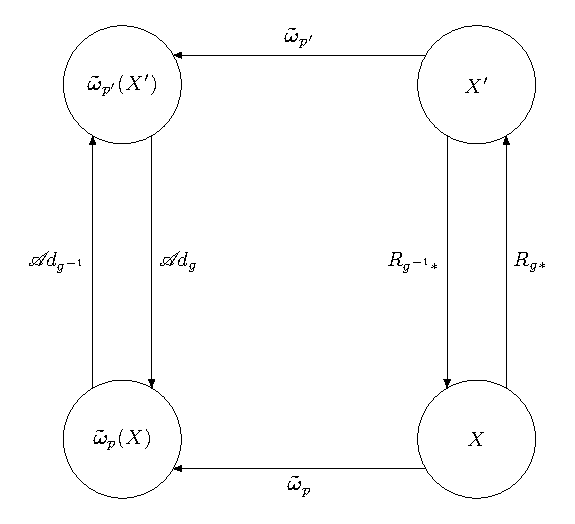
\includegraphics[width=0.5\textwidth]{../tikzpicture/I21}
      \caption{形式场给出的矢量空间的联系}
      \label{fig:I-2-1}
    \end{figure}

    也就是说如图\ref{fig:I-2-1}所示,$\bm{\tilde{\omega}}_{p'}(X')$ 有两种途径得到,这也是式\ref{eq:I-2-3}所要表达
    的含义,我们知道推前映射$R_{g*}$是线性映射,且$\dim{X} = \dim{X'}$,也就是说$X$和 $X'$是同构的矢量空间,而$\bm{\tilde{\omega}}_p(X)$ 和$\bm{\tilde{\omega}}_p'(X')$都是$G$的恒等元的矢量空间,彼此之间也同构,
    所以我们可以给出关系\[
      \bm{\tilde{\omega}}_p(R_{g^{-1}*} X') = \mathscr{A}\!d_{g}\bm{\tilde{\omega}}_{p'}(X')  
    .\] 
    代入式子\ref{eq:I-2-2}有,注意式子\ref{eq:I-2-2}反应p和p'之间关系的群元是$g'$
    \begin{align*}
      \mathscr{A}\!d_{g^{-1}}\bm{\tilde{\omega}}_{p'g'^{-1}}(R_{g'^{-1}*}X')& = \mathscr{A}\!d_{g^{-1}}\bm{\tilde{\omega}}_p(R_{g'^{-1}*}X') = \mathscr{A}\!d_{g^{-1}}\mathscr{A}\!d_{g'}\bm{\tilde{\omega}}_{p'}(X')\\& = \mathscr{A}\!d_{g^{-1}g'} \bm{\tilde{\omega}}_{p'}(X') = \mathscr{A}\!d_{(g'^{-1}g)^{-1}}\bm{\tilde{\omega}}_{p'}(X')
    \end{align*}
    最后,结合上面所有讨论我们给出\[
    \bm{\tilde{\omega}}_{p'g'^{-1}g}R_{g'^{-1}g*}X' = \mathscr{A}\!d_{(g'^{-1}g)^{-1}}\bm{\tilde{\omega}}_{p'}(X')
    .\] 
    而$p'g'^{-1}g = pg$,也就是说与$p$联系的两点 $p',pg$可以给出条件2的式子,而与 $p$ 同fiber的所有点都有联系,也就是说所有的点都有条件2'给出的关系,也就是条件2成立

    下面我们正式证明定义\ref{def:联络-1}和定义\ref{def:联络-2}等价,给出定理
     \begin{theorem}
       {}{I-2-1} 
       定义\ref{def:联络-1}和定义\ref{def:联络-2}等价
    \end{theorem}
    \begin{proof}
      (定义\ref{def:联络-2} $\Rightarrow$ 定义$\ref{def:联络-1}$) 设$\bm{\tilde{\omega}} $ 是定义 \ref{def:联络-2}的联络,就可以给每一$p\in P$的切空间$T_pP$定义如下的线性水平子空间 
      \[
        H_p := \{X \in T_pP \mid \bm{\tilde{\omega}}_p(X) = 0\})  
      .\] 
      \begin{enumerate}
        \item \textbf{定义}\ref{def:联络-2}$\bm{\Rightarrow T_pP = V_p \oplus H_p, \quad \forall p \in P} :$我们令$A \equiv \bm{\tilde{\omega}}_p(X) \in \mathscr{G}$则有$X_1 \equiv A^*_p \in V_p $,再令$X_2 \equiv X - A^*_p$,则 \[
            \bm{\tilde{\omega}}_p(X_2) =\bm{\tilde{\omega}}_p(X) - \bm{\tilde{\omega}}_p(A^*_p) =  A - A = 0
        .\] 
        \begin{note}
          第一步是因为$l$形式场本质上是 $(0,l)$型张量,结合张量的定义,可知 $\bm{\tilde{\omega}}_p$ 是线性的,第二步用了\ref{def:联络-2}的条件1
        \end{note}
        所以$X_2 \in H_p$,由$X_2 \equiv X -A^*_p$得 $X = X_1 +X_2$,下面我们来说明分解的唯一性,每有一个$X$便会给出一个 $A$,也就是说一一性成立,也就是说$X \mapsto A$是唯一的,再根据上面的步骤,不难得到
         $X_2$亦是唯一的,也就是说分解具有唯一性.
       \item \textbf{定义}\ref{def:联络-2}$\bm{\Rightarrow R_{g*}[H_p] = H_{pg},\quad \forall p\in P, g \in G :}$ 
         设$X \in H_p$,则有 \[
           \bm{\tilde{\omega}}_{pg}{R_{g*}X} = \mathscr{A}\!d_{g^{-1}}\bm{\tilde{\omega}}_p(X) = \mathscr{A}\!d_{g^{-1}}0 = 0 \Rightarrow R_{g*}X \in H_{pg} 
         .\] 
         所以$R_{g*}[H_p]\subset H_{pg}$,现在令$Y \in H_{pg}$,重复上面步骤\[
           \bm{\tilde{\omega}}_{p}{R_{g^{-1}*}Y} = \mathscr{A}\!d_{g}\bm{\tilde{\omega}}_{pg}(X) = \mathscr{A}\!d_{g}0 = 0 \Rightarrow R_{g^{-1}*}Y \in H_{p} 
         .\] 则$R_{g^{-1}*} [H_{pg}] \subset H_p$,故$H_p = H_{pg}$
       \item $H_p$光滑地依赖于 $p$由 $\bm{\tilde{\omega}}$是$C^\infty$ 来保证.
         \begin{note}
           还是来一点hand-waving,$H_p$是光滑地依赖于p,也就是说可以在 $p$上定义一个 $C^\infty$的矢量场,而$\bm{\tilde{\omega}}$ 可以把$X$映射到 $\mathscr{G}$和$H_p$, $\bm{\tilde{\omega}}$的 $C^\infty$保证了两个矢量空间是光滑的,
           从侧面应证了,$X$在 $p$的邻域上是光滑的.
         \end{note}
      \end{enumerate}
      (定义\ref{def:联络-1} $\Rightarrow$ 定义$\ref{def:联络-2}$)在这里我们只要找到$\bm{\tilde{\omega}} \in \Lambda_p(1,\mathscr{G})$满足定义\ref{def:联络-2}的要求即可,根据定义\ref{def:联络-1}
      $\forall X \in T_pP,\exists $唯一的$X_1 \in V_p,X_2 \in H_p$满足$X = X_1 + X_2$. $X_1\in  V_p \Rightarrow \exists \text{唯一} A\in \mathscr{G}\text{满足},X_1 = A^*_p$,故$X = A^*_p + X_2$,定义
       \begin{equation}
         \bm{\tilde{\omega}}_{p} (X) = \bm{\tilde{\omega}}_{p}(A^*_p + X_2):=A \quad  \forall p \in P
         \label{eq:I-2-4}
      \end{equation}
      $\bm{\tilde{\omega}}$的 $C^\infty$由定义\ref{def:联络-1}第三条保证,我们来验证满足定义\ref{def:联络-2}要求
      \begin{enumerate}
        \item 由式\ref{eq:I-2-4}得$\bm{\tilde{\omega}}_p(A^*_p) = A $;
        \item  因为 $\bm{\tilde{\omega}} $是线性的,所以只需要证明$\bm{\tilde{\omega}}_p(X_1)$和$\bm{\tilde{\omega}}_p(X_2)$满足即可
          ,由定义\ref{def:联络-1}条件2知道$R_{g*}  \in  H_{pg}$,所以$ \bm{\tilde{\omega}}_p(X_2) = 0, \bm{\tilde{\omega}}_{pg}(R_{g*}X_2) = 0 $,不难给出\[
            \bm{\tilde{\omega}}_{pg}(R_{g*}X_2) = \mathscr{A}\!d_{g^{-1}}\bm{\tilde{\omega}}_p(X_2)
          .\] 
          对于$\bm{\tilde{\omega}}_p(X_1)$有
           \begin{align*}
             \bm{\tilde{\omega}}_{pg}(R_{g*}X_1)& = \bm{\tilde{\omega}}_{pg}(R_{g*}A^*_p) = \bm{\tilde{\omega}}_{pg}[\mathscr{A}\!d_{g^{-1}}A)^*_{pg}] \quad \text{第二个等号用到定理}\ref{thm:I-1-7}\\
                                                & = \mathscr{A}\!d_{g^{-1}}A = \mathscr{A}\!d_{g^{-1}}\bm{\tilde{\omega}}_{p}(A^*_p) \quad \text{这两步是定义\ref{def:联络-2}条件1(已经验证过了)}\\
                                                & = \mathscr{A}\!d_{g^{-1}}\bm{\tilde{\omega}}_p{X_1}
          .\end{align*}
      \end{enumerate}
    \end{proof}
    \begin{definition}
      {Connection(3)}{联络-3} 
      主丛$P(M,G)$的一个 \textbf{联络}是对每个局域平凡$T_U:\pi^{-1}[U] \rightarrow U \times G,U\subset M$指定一个$U$上的
      $C^\infty$的$\mathscr{G}$值的1形式场$\bm{\omega}_U$.如果 $T_V:\pi^{-1}[V] \to  V\times G$是另一局域平凡,$U \cap V \neq \varnothing$,从$T_U$到 $T_V$的转换函数为 $g_{UV}$,则还要求
       \[
         \bm{\omega}_V(Y)= \mathscr{A}\!d_{g_{UV}(x)^{-1}}\bm{\omega}_U(Y) + L^{-1}_{g_{UV}(x)*}g_{UV*}(Y),\quad \forall x \in U\cap V, Y \in T_xM 
      .\] 
    \end{definition}
    我们来理解一下这个等式,$\mathscr{A}\!d_{g_{UV}(x)^{-1}}\bm{\tilde{\omega}}_U(Y)$是李代数元,不难猜想$L^{-1}_{g_{UV}(x)*}g_{UV*}(Y)$也是李代数元,事实上确实是,我们可以根据图\ref{fig:I-2-2}看出它们之间的关系.
    (注意红色部分与蓝色部分的联系)
    \begin{figure}[htpb]
      \centering
      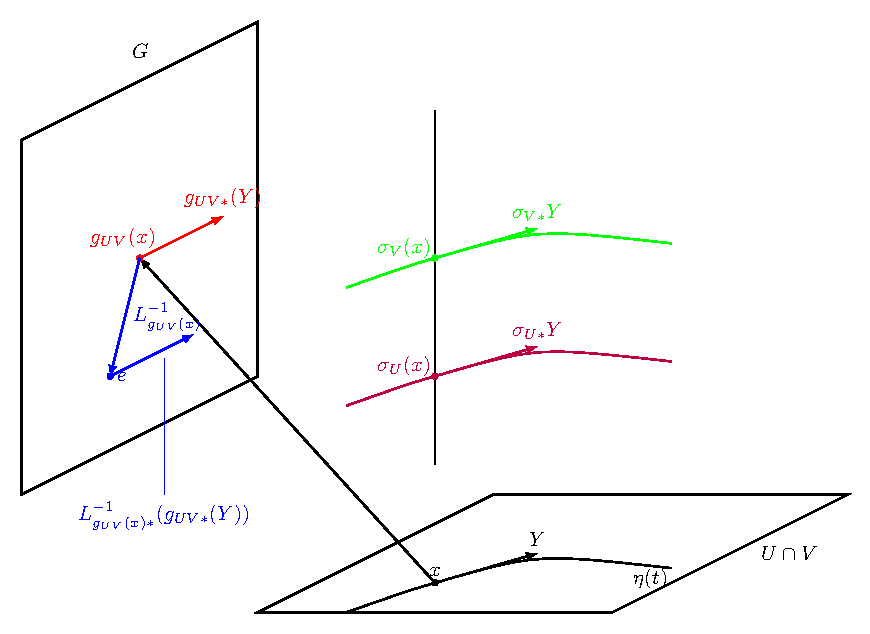
\includegraphics[width=0.8\textwidth]{../tikzpicture/I22.pdf}
      \caption{定义\ref{def:联络-3}配套图}
      \label{fig:I-2-2}
    \end{figure}
    \begin{theorem}
      {}{I-2-2}
      定义\ref{def:联络-2}和定义\ref{def:联络-3}等价.
    \end{theorem}
    \begin{proof}
      (定义\ref{def:联络-2}$\Rightarrow$定义\ref{def:联络-3}) 由定义\ref{def:联络-2}知道主丛上有$\bm{\tilde{\omega}}\in \Lambda_P(1, \mathscr{G}) $,我们需要给底流形定义$\bm{\omega}_U \in \Lambda_U(1,\mathscr{G}) $,
      定义\ref{def:联络-3}要求在局域平凡U上指定形式场,根据\ref{thm:I-1-3}可以给出$\sigma_U:U \to P$给出一个与$T_U$定义的局域截面,根据拉回映射的定义可以给出 $U$上的1形式场.
       \begin{note}
       拉回映射:假设存在两个流形$M$和 $N$,流形之间存在光滑映射$\phi:M \to N$,且在$N$存在 $l$形式场,定义 $M$上的 $l$形式场,并记作 $\phi^*:\mathscr{F}_N(0,l) \to \mathscr{F}_M(0,l)$,假设$\forall T \in \mathscr{F}_N(0,l)$定义$\phi^*T \in \mathscr{F}_M(0,l)$为\[
         (\phi^*T)_{a_1 \cdots a_l} \mid _p (v_1)^{a_1} \cdots (v_l)^{a_l} := T_{a_1 \cdots a_l} \mid_{\phi_p}(\phi_* v_1)^{a_1} \cdots (\phi_*v_l)^{a_l}, \quad \forall  p \in M, v_1, \cdots ,v_l \in V_p 
       .\] 简而言之,就是借助了$N$上的形式场,给了 $M$上的形式场,更多详细内容参考书P102.
      \end{note}
      就是说给出$\bm{\omega}_U \equiv \sigma_U^* \bm{\tilde{\omega}}  $ 是$U$上 $C^\infty$的$\mathscr{G}$值的$1$形式场,而如果给定另一个底流形 $V$,且 $U \cap V \neq \varnothing$,故在$U \cap V$的区域内还能给出$\bm{\omega}_V \equiv \sigma^*_V \bm{\tilde{\omega}}$,我们在前面给出转换函数是要求 $x \in U\cap V$,给出$\sigma_U(x)$和 $\sigma_V(x)$的认同,这里我们应该给出相同的要求.

      我们来看它们之间满足的关系
      \begin{equation*}
        \bm{\omega}_V \mid _x(Y)  = (\sigma^*_V \bm{\tilde{\omega}} \mid _{\sigma_V(x)})(Y) = \bm{\tilde{\omega}} \mid _{\sigma_V(x)}(\sigma_{V*}Y)
      \end{equation*}
      我们来看$\sigma_{V*}Y$和$\sigma_{U*}Y$的关系,其中$\eta(t)$是过 $x$的 $C^\infty$曲线,满足$\eta(0) = x, \left.\frac{d}{dt}\right|_{t=0} \eta(t) = Y$
       \begin{align*}
         \sigma_{V*}Y & = \sigma_{V*}\left.\frac{d}{dt}\right|_{t = 0}\eta(t) =\left.\frac{d}{dt}\right|_{t = 0}(\sigma_V \eta(t)) =\left.\frac{d}{dt}\right|_{t = 0}(\sigma_U(\eta(t))g_{UV}(\eta(t)))\quad \text{最后一个等号见式}\ref{eq:I-1-2}\\
                      &=\sigma_U(\eta(0))\left.\frac{d}{dt}\right|_{t = 0}g_{UV}(\eta(t)) + [\left.\frac{d}{dt}\right|_{t = 0}(\sigma_U(\eta(t)))][g_{UV}(\eta(0))]\\
                      &=\sigma_U(x)\left.\frac{d}{dt}\right|_{t = 0}g_{UV}(\eta(t)) + [\left.\frac{d}{dt}\right|_{t = 0}(\sigma_U(\eta(t)))][g_{UV}(x)]\\
                                                &=\left.\frac{d}{dt}\right|_{t = 0} \sigma_U(x)g_{UV}(\eta(t)) )+ \left.\frac{d}{dt}\right|_{t = 0}(\sigma_U(\eta(t)))g_{UV}(x) \quad \text{这一步只是把$\sigma_U(x),g_{UV}(x)$当作常数}
             .\end{align*}
我们分开计算上式,先来看第一项,首先有\[
  \sigma_U(x)g_{UV}(\eta(t)) = \sigma_V(x) g_{UV}(x)^{-1}g_{UV}(\eta(t)) = \sigma_V(x) L_{g_{UV}(x)^{-1}}g_{UV}(\eta(t)) = R_{\sigma_V(x)}[L^{-1}_{g_{UV}(x)}g_{UV}(\eta(t))]
.\] 
则
\begin{align*}
  \left.\frac{d}{dt}\right|_{t = 0} \sigma_U(x)g_{UV}(\eta(t))& = \left.\frac{d}{dt}\right|_{t = 0} R_{\sigma_V(x)}[L^{-1}_{g_{UV}(x)}g_{UV}(\eta(t))]\\
                                                              & =R_{\sigma_V(x)*}L^{-1}_{g_{UV}(x)*}g_{UV*}\left. \frac{d}{dt}\right|_{t = 0} \eta(t)\\
                                                              & = R_{\sigma_V(x)*}L^{-1}_{g_{UV}(x)*}g_{UV*}(Y)\\
                                                              & =[L^{-1}_{g_{UV}(x)*}g_{UV*}(Y)]^*_{\sigma_V(x)} \quad \text{定义}\ref{def:基本矢量场}
.\end{align*}
再来看第二项
\begin{align*}
  \left.\frac{d}{dt}\right|_{t = 0}(\sigma_U(\eta(t)))g_{UV}(x) &= \left.\frac{d}{dt} \right|_{t = 0}(R_{g_{UV}(x) }\sigma_U(\eta(t)))\\
                                                                & = (R_{g_{UV(x)*}})\left.\frac{d}{dt} \right|_{t = 0} \sigma_U(\eta(t))\\
                                                                & = (R_{g_{UV(x)*}})(\sigma_{U*})\left.\frac{d}{dt} \right|_{t = 0} \eta(t)\\
                                                                &= R_{g_{UV}(x)*}\sigma_{U*}Y
.\end{align*}
所以我们有
\begin{equation}
  \sigma_{V*}Y =  R_{g_{UV}(x)*}\sigma_{U*}Y + [L^{-1}_{g_{UV}(x)*}g_{UV*}(Y)]^*_{\sigma_V(x)}
  .\label{eq:I-2-6}
\end{equation}
我们回到$\bm{\omega}_V|_x(Y)$,我们有
\begin{align*}
  \bm{\omega}_V|_x(Y)& =\bm{\tilde{\omega}}|_{\sigma_V(x)}[R_{g_{UV}(x)*}\sigma_{U*}Y + [L^{-1}_{g_{UV}(x)*}g_{UV*}(Y)]^*_{\sigma_V(x)}]\\
                     & = \bm{\tilde{\omega}}|_{\sigma_V(x)}[R_{g_{UV}(x)*}\sigma_{U*}Y ]+\bm{\tilde{\omega}}|_{\sigma_v(x)}[[L^{-1}_{g_{UV}(x)*}g_{UV*}(Y)]^*_{\sigma_V(x)}]\\
                     & = \bm{\tilde{\omega}}|_{\sigma_U(x)g_{UV}(x)}[R_{g_{UV}(x)*}\sigma_{U*}Y ] +L^{-1}_{g_{UV}(x)*}g_{UV*}(Y)\\
                     & = \mathscr{A}\!d_{g_{UV}(x)^{-1}}\bm{\tilde{\omega}}_{\sigma_U(x)}(\sigma_{U*}Y)+ L^{-1}_{g_{UV}(x)*}g_{UV*}(Y)\\
                     & = \mathscr{A}\!d_{g_{UV}(x)^{-1}}\bm{\omega}_{U}|_x(Y)+ L^{-1}_{g_{UV}(x)*}g_{UV*}(Y)\\
.\end{align*}
就是我们定义\ref{def:联络-3}的要求,证明结束.

(定义\ref{def:联络-3} $\Rightarrow$ 定义 \ref{def:联络-2}),也就是有$\bm{\omega}_U \in \Lambda_U(1,\mathscr{G}) $,求$\bm{\tilde{\omega}} \in \Lambda_p(1,\mathscr{G})$ 

1. 首先在$\pi^{-1}[U]$上定义一个$\mathscr{G}$值上的1形式场$ \bm{\tilde{\omega}} $,由于只定义了$\pi^{-1}[U]$上的形式场,所以这里记作$\bm{\tilde{\omega}}^U $ 以作区别,对于$\forall $一点$x \in U$,令$p \equiv \sigma_U(x)$
,而对p的任一矢量$X$,令 $Y \equiv \pi_* X, Z \equiv X - \sigma_{U*} Y$,故
\begin{align*}
  \pi_*Z = \pi_* X -  \pi_* \sigma_{U*} Y = \pi_* X - (\pi \circ \sigma)_* Y = Y - Y = 0
\end{align*}
\begin{note}
 注意 $\pi$是一个多对一的映射, $\sigma$只会把 $x$映射到 $p$点,也就是说 $(\pi \circ \sigma_U)$恒为 $e$,而 $(\sigma_U \circ \pi)$只有作用到 $p$点才为 $e$. 
\end{note}
即$Z \in V_p$是竖直子空间,故由定理\ref{thm:I-1-4},$V_p,\mathscr{G}$内的矢量存在一一对映的关系,即$\exists  A \in \mathscr{G}$,满足$Z = A^*_p$,于是 \[
  X = A^*_p + \sigma_{U*}Y
.\] 
我们给出$\pi^{-1}[U]$上的定义
\begin{align*}
  \bm{\tilde{\omega}}^U| _p(X) =  \bm{\tilde{\omega}}^U| _p(A^*_p + \sigma_{U*}Y) := A + \bm{\omega}_U |_{\pi(p)}(Y)  
.\end{align*}
对于其它不在截面的点,但是与$p$同fiber的点 $p' \in \pi^{-1}[y]$, 且$X'$为其切矢量,有唯一的$g\in G$使得$p' = pg$则$\bm{\tilde{\omega}}^U $ 在$p'$点的定义 为
\begin{align*}
  \bm{\tilde{\omega}}^U| _{p'}(X') := \mathscr{A}\!d_{g^{-1}}\bm{\tilde{\omega}}^U|_p(R_{g^{-1}*}X') 
.\end{align*}
\begin{note}
  不在fiber的点$p'$的定义是迎合定义\ref{def:联络-2}要求给出的,下面证明确实满足定义\ref{def:联络-2}
\end{note}

2.我们需要验证上面定义是否满足 定义\ref{def:联络-2}的要求,定义\ref{def:联络-2}要求两点,我们来看第一点,对于截面上的点有:
 \begin{align*}
 \bm{\tilde{\omega}}^U(A^*_p) =  \bm{\tilde{\omega}}^U(A^*_p + 0 ) = A + 0 = A
.\end{align*}
对于不是截面上的点但和$p$同fiber的点有
\begin{align*}
  \bm{\tilde{\omega}}^U|_{p'}(A^*_{p'}) &= \mathscr{A}\!d_{g^{-1}}\bm{\tilde{\omega}}^U|_p(R_{g^{-1}*}A^*_{p'}) \\
                                        & = \mathscr{A}\!d_{g^{-1}}\bm{\tilde{\omega}}^U|_p (\mathscr{A}\!d_{g}A)^*_{p} \quad \text{定理}\ref{thm:I-1-7}\\
                                        & = \mathscr{A}\!d_{g^{-1}}\mathscr{A}\!d_{g}A\\
                                        &=A
.\end{align*}
第一点满足,接下来看第二点
\begin{align}
  \bm{\tilde{\omega}}^U_{pg}(R_{g*}X) = \mathscr{A}\!d_{g^{-1}} \bm{\tilde{\omega}}^U_p[(R_{g^{-1}*})(R_{g*}X)] = \mathscr{A}\!d_{g^{-1}}\bm{\tilde{\omega}}^U_p(X) \label{eq:I-2-5}
.\end{align}
根据式\ref{eq:I-2-5},我们给出了截面上的点与其同fiber的点的关系满足定义\ref{def:联络-2}第二条的要求,但是定义\ref{def:联络-2}要求的p是任意点,也就是说
我们还需要验证不在截面上的两点之间满足定义\ref{def:联络-2}的要求.事实上我们在前文中证明过相同的问题,详情请见图\ref{fig:I-2-1}所在位置附近的证明.
\begin{note}
  事实上,定义\ref{def:联络-2}有一个等价条件,观察式\ref{eq:I-2-5},满足等价条件.
\end{note}
由此可见,在 $\pi^{-1}[U]$上我们定义的$\bm{\tilde{\omega}}^U $ 满足定义\ref{def:联络-2}的要求.

3.前文给出的是底流形$M$上的 $U$的形式场,在底流形再指定一个 $V$满足 $U\cap V$,在$\pi^{-1}[U\cap V]$上有形式场$\bm{\tilde{\omega}}^U $ 和$\bm{\tilde{\omega}}^V $ 两个形式场,只有
让 \[
\bm{\tilde{\omega}}^V = \bm{\tilde{\omega}}^U  
.\] 
才能给出全局的统一的形式场并且满足定义\ref{def:联络-2}的要求.根据图\ref{fig:I-2-1}中由$R_{g*}$诱导的矢量空间是同构的,而 $\mathscr{A}\!d_{g^{-1}}$诱导的矢量空间亦是同构的,那么
对于目前而言,一个$X$有两个 形式场 $\bm{\tilde{\omega}}^V $ 和$\bm{\tilde{\omega}}^U $,要想证明其相等,只需要在一点上证明其相等,随后根据$R_{g*}$和 $\mathscr{A}\!d_{g^{-1}}$ 便可以令$U\cap V$的形式场相等.重复上述步骤
可以给出全局统一的形式场.

在$\pi^{-1}[U\cap V]$区域内,每条fiber上有两个局域截面的点分别由$U$和 $V$给出,不妨记作 $p = \sigma_U(x)$和$p' = \sigma_V(x)$它们之间满足 \[
  \sigma_V(x) = \sigma_U(x)g_{UV}\Rightarrow(g_{UV}\text{记作}g) p' = pg
.\]下面我们来证明$\bm{\tilde{\omega}}^V = \bm{\tilde{\omega}}^U  $,选择证明$p'$点,由于$X' = A^*_{pg} + \sigma_{V*}Y$,则只需要证明 \[
\bm{\tilde{\omega}}^V_{pg}( A^*_{pg} + \sigma_{V*}Y) = \bm{\tilde{\omega}}^U_{pg}(A^*_{pg} + \sigma_{V*}Y)
.\] 
即只需要\[
\bm{\tilde{\omega}}^V_{pg}(  \sigma_{V*}Y) = \bm{\tilde{\omega}}^U_{pg}( \sigma_{V*}Y)
.\] 
而$\sigma_{V*} $和$ \sigma_{U*}$ 之间的关系我们在上文证明过,关系式是式\ref{eq:I-2-6},不同式子的含义可见图\ref{fig:I-2-2},则
\begin{align*}
  \bm{\tilde{\omega}}^U_{pg}( \sigma_{V*}Y) &=  \bm{\tilde{\omega}}^U_{pg}( R_{g_{UV}(x)*}\sigma_{U*}Y + [L^{-1}_{g_{UV}(x)*}g_{UV*}(Y)]^*_{\sigma_V(x)})\\
  & = \bm{\tilde{\omega}}^U_{pg}( R_{g_{UV}(x)*}\sigma_{U*}Y )+ \bm{\tilde{\omega}}^U_{pg}([L^{-1}_{g_{UV}(x)*}g_{UV*}(Y)]^*_{\sigma_V(x)})\\
  & = \mathscr{A}\!d_{g^{-1}} \bm{\tilde{\omega}}_p(\sigma_{U*}Y) +  L^{-1}_{g_{UV}(x)*}g_{UV*}(Y)\\
  & =  \mathscr{A}\!d_{g^{-1}}\bm{\omega}_U(Y) + L^{-1}_{g_{UV}(x)*}g_{UV*}(Y)\\
  & = \omega_V(Y) \quad \text{定义}\ref{def:联络-3}
.\end{align*}
且\[
\bm{\tilde{\omega}}^V_{pg}(  \sigma_{V*}Y) = \bm{\omega}_V(Y) 
.\]
故 $\bm{\tilde{\omega}}^V_{pg}(  \sigma_{V*}Y) = \bm{\tilde{\omega}}^U_{pg}( \sigma_{V*}Y)$命题得证.
\end{proof}

以上我们给出了关于联络的三个等价定义.上面都是比较抽象的定义,我们把它应用到更具体的环境中,如果结构群是矩阵群的话,我们有如下定理:
\begin{theorem}
  {}{I-2-3}
  若结构群G是矩阵群,则$\bm{\omega}_V $ 和$\bm{\omega}_U $ 的关系可以写作\[
    \bm{\omega}_V = g_{UV}^{-1}\bm{\omega}_U g_{UV}^{} + g_{UV}^{-1} d g_{UV}^{}
  .\] 
\end{theorem}
\begin{note}
  G是矩阵群意思是它的元素是$N \times N$矩阵,故其李代数元也是 $N\times N$矩阵,令$\mathscr{V} \equiv \left\{ N\times N \right\} $,则$\mathscr{V}$是矢量空间,
  且$G \subset \mathscr{V},\mathscr{G}\subset \mathscr{V}$,而 $\bm{\omega}_U $ 和$\bm{\omega}_V $ 都是$\mathscr{G}$值的$1$ 形式场,即$\bm{\omega}_U,\bm{\omega}_V \in \Lambda_{U\cap V}(1,\mathscr{V})$,而$g_{UV}:U\cap V \rightarrow G \subset \mathscr{V}$是作用到底流形上的一个点上,即$g_{UV} \in \Lambda_{U\cap V}(0,\mathscr{V})$,同理 $g_{UV}^{-1}(x)$是$g_{UV}(x)$的逆矩阵所以 $g_{UV} ^{-1}(x)$依旧是$\Lambda_{U\cap V}(0,\mathscr{V})$
  ,所以定理\ref{thm:I-2-3}的等式是$1$形式场等式.
\end{note}
\begin{proof}
  对于$\bm{\omega}_U $ 和$\bm{\omega}_V $ 有通用的等式\[
    \bm{\omega}_V(Y) = \mathscr{A}\!d_{g_{UV}^{}(x)^{-1}}\bm{\omega_U}(Y) + L^{-1}_{g_{UV}^{}(x)*}g_{UV*}^{}(Y) 
  .\] 
  我们简化一下写法令$g = g_{UV}^{}(x)$, $A = \bm{\omega}_U(Y) \in \mathscr{G}$,则对于等号左边第一项有
  \begin{align*}
    \mathscr{A}\!d_{g_{UV}^{}(x)^{-1}}\bm{\omega_U}(Y) &= \mathscr{A}\!d_{g^{-1}}A = g^{-1}Ag\quad \text{来源于定理}\ref{thm:G-8-1}\text{对两边求导并令}t = 0\\
                                                       & = g_{UV}^{}(x)^{-1}\bm{\omega}_U(Y)g_{UV}(x) 
  .\end{align*}
  对于等号左面第二项
  \begin{align*}
    L^{-1}_{g_{UV}^{}(x)*}g_{UV*}^{}(Y) &=   L^{-1}_{g_{UV}^{}(x)*}g_{UV*}^{}(\left. \frac{d}{dt}  \right|_{t = 0} \eta(t) )\\
                                        & = \left. \frac{d}{dt}  \right|_{t = 0}L^{-1}_{g_{UV}^{}(x)}g_{UV}^{}( \eta(t) )\\
                                        & = \left. \frac{d}{dt}  \right|_{t = 0}g_{UV}^{}(x)^{-1}g_{UV}^{}( \eta(t) )\\
                                        & = g_{UV}^{}(x)^{-1}\left. \frac{d}{dt}  \right|_{t = 0}g_{UV}^{}( \eta(t) )\\
  .\end{align*}
  目前比较容易,下面需要一些技巧,首先$g_{UV} \in \Lambda_{U\cap V}(0,\mathscr{V})$,则$d g_{UV} \in \Lambda_{U\cap V}(1,\mathscr{V})$,以$\left\{ e_r \right\} $ 代表$\mathscr{V}$的一组基矢量,则有\[
    g_{UV} = e_r f^r, dg_{UV} = e_r df^r 
  .\] 故
  \begin{align*}
    L^{-1}_{g_{UV}^{}(x)*}g_{UV*}^{}(Y) & = g_{UV}^{}(x)^{-1}\left. \frac{d}{dt}  \right|_{t = 0}g_{UV}^{}( \eta(t) )\\
                                        & = g_{UV}^{}(x)^{-1}\left. \frac{d}{dt}  \right|_{t = 0}e_r f^r(\eta(t))\\
                                        & = g_{UV}^{}(x)^{-1}e_r\left. \frac{d}{dt}  \right|_{t = 0} f^r(\eta(t))\\
  .\end{align*}
  我们观察$\left. \frac{d}{dt}  \right|_{t = 0} f^r(\eta(t))$ ,$f^r$是 $\mathbb{R} or \mathbb{C}$的0形式场,回顾切矢的定义不难给出\[
  \left. \frac{d}{dt}  \right|_{t = 0} f^r(\eta(t)) = Y(f^r) = df^r(Y)
  .\] 
  \begin{note}
    切矢的定义为流形上的$C^1$曲线(至少连续)上面定义了函数(0形式场),线可以使用参数式 $C(t)$来表示,定义的切矢为 \[
      T(f) := \left.\frac{d(f(C(t)))}{dt} \right|_{t_0} 
    .\] T就是在$t_0$点$f^r$的切矢. f还会给出对偶矢量场,定义为 \[
   df(v) := v(f) 
    .\] 由于$df$是作用于1个矢量,故其为1形式场.
  \end{note}
由此可见
\begin{align*}
     L^{-1}_{g_{UV}^{}(x)*}g_{UV*}^{}(Y)& = g_{UV}^{}(x)^{-1}e_r\left. \frac{d}{dt}  \right|_{t = 0} f^r(\eta(t))\\
                                        & = g_{UV}(x)^{-1}dg_{UV}^{}(Y)
.\end{align*}
\end{proof}
总结上述证明有\[
\bm{\omega}_V(Y) = g_{UV}^{}(x)^{-1}\bm{\omega}_U(Y)g_{UV}(x) + g_{UV}(x)^{-1}dg_{UV}^{}(Y)
.\] 
由于$x$是确定的点,上述式子表述的是作用于 $x$点的切矢量 $Y$,故可以简记为 \[
\bm{\omega}_V = g_{UV}^{-1}\bm{\omega}_U(Y)g_{UV} + g_{UV}^{-1}dg_{UV}^{}
.\] 
\section{用标架计算曲率张量(Frame Method For Computing Curvature)}
为了更好的进行下一节的内容,这里补充一节,来源于书中选读5.7节,P140.本节讨论如何利用标架计算曲率.

我们给定流形$M$,并在上面定义了导数算符 $\nabla_a$,设$\{(e_\mu)^a\}$是任一基底场,定义域为$U \subset M$,其第$\mu$基矢场 $(e_\mu)^a$沿第 $\tau$基矢场 $(e_\tau)^a$的导数依旧为U上的矢量场,可借基底场$\{(e_\sigma)^a\}$展开,写作下式 
\begin{equation}
  (e_\tau)^b\nabla _b(e_\mu)^a = \gamma^{\sigma}{}_{\mu\tau}(e_\sigma)^a 
  \label{eq:I-2-7}
\end{equation}
展开系数$\gamma^\sigma_{\mu\tau}$称为 \textbf{联络系数(connection coefficients)},如果基底场是坐标基底场的话,则有
\begin{equation}
  (\frac{\partial   }{\partial x^\tau} )^b \nabla_b (\frac{\partial   }{\partial x^\mu} )^a = \Gamma^\sigma{}_{\mu\tau}(\frac{\partial   }{\partial x^\sigma} )^a =\Gamma^{a}{}_{\mu\tau} 
  \label{eq:I-2-8}
\end{equation}
这里我们使用了和克氏符相同的符号$\Gamma^\sigma{}_{\mu\tau}$,是因为上式给出的那组数确实是克氏符在坐标基底场的分量,我们借助这个证明来回顾一下克氏符的定义以及曲率的相关知识点.

我们在第3章给出的克氏符定义的式子为(来源p74,定理3-1-5)\[
\nabla_av^b = \partial_av^b + \Gamma^{b}{}_{ac}v^c 
.\] 
即$\Gamma^{b}{}_{ac}v^c = \nabla_a v^b -\partial_a v^b$,我们选择坐标基底场作为$v^a = (\frac{\partial   }{\partial x^\sigma} )^a$,可以给出 \[
\Gamma^{b}{}_{ac}v^c = \nabla_a v^b -\partial_a v^b = \nabla_a v^b 
.\] 
最后一个括号是因为选定坐标基矢就不会改变,随后我们调整指标位置为\[
\Gamma^{a}{}_{bc}v^c = \nabla_b v^a \Rightarrow  \Gamma^{a}{}_{bc}(\frac{\partial}{\partial x^\mu} )^c = \nabla_b (\frac{\partial   }{\partial x^\mu} )^a
.\]
\begin{note}
 这里在代入指标,原则上$v^a$和 $v^b$内部代入的指标应该有两项,在这里会有细微的差别,原因在于左侧 $v^c$ 是哑指标,而 $v^a$和 $v^c$是同一个矢量,为了指标平衡,给出的上式.
\end{note}
两边左乘$(\frac{\partial   }{\partial x^\tau})^b$,给出\[
  (\frac{\partial   }{\partial x^\tau} )^b \nabla_b (\frac{\partial   }{\partial x^\mu} )^a = (\frac{\partial   }{\partial x^\tau})^b\Gamma^{a}{}_{bc}(\frac{\partial}{\partial x^\mu} )^c = \Gamma^{a}{}_{\tau\mu} = \Gamma^{a}{}_{\mu\tau}  
.\] 
由此可见当代入坐标基矢后,式\ref{eq:I-2-8}给出的式子确实是克氏符的那组数.可以作为克氏符的等价定义.
\begin{note}
  式\ref{eq:I-2-8}指标存在一些问题,但是由于导数算符的无挠性指标确实可以交换位置,但是为什么这么写,未知? 
\end{note}
让我们把思路回到非基底场的情况上,也就是式\ref{eq:I-2-7},使用$(e^\nu)_a$作用到式 \ref{eq:I-2-7}可以给出 \[
\gamma^{\nu}{}_{\mu\tau} =(e^\nu)_a  (e_\tau)^b\nabla _b(e_\mu)^a
.\] 
我们定义$\nabla _a$在基底场$\left\{ (e_\mu)^a \right\} $ 的联络1形式场,简记为$\omega_\mu{}^{\nu}{}_{a}$,定义是\[
  \omega_\mu{}^{\nu}{}_{a} := -\gamma^{\nu}{}_{\mu\tau}(e^\tau)_a
.\] 
\begin{note}
  实际上$\gamma^{\nu}{}_{\mu \tau}$ 是下一节中的联络形式场,这里这么定义是为了凑出嘉当第二结构方程的形式,具体内容见书上P1108 选读I-2-1最后一段.这里交换$\mu ,\nu$指标就是会带来一个负号,原因是因为\[
 - (e^\nu)_c \nabla _a(e_\mu)^c = (e_\mu)^c\nabla_a(e^\nu)_c 
.\]借鉴于式子\ref{eq:I-2-9},同样有帮助于理解的还有式子\ref{eq:I-2-11}
\end{note}
这里$\mu,\nu$的取值均为 $1 \cdots n$,也就是说这里我们有 $n^2$个1形式场,称为\textbf{联络1形式(Connection 1 Form)},代入$\gamma^{\nu}{}_{\mu\tau}$ 有
\begin{equation}
  \omega_\mu{}^{\nu}{}_{a} := -(e^\tau)_a(e^\nu)_c(e_\tau)^b\nabla _b(e_\mu)^c = - \delta^{b}{}_{a}(e^\nu)_c \nabla_b(e_\mu)^c = - (e^\nu)_c \nabla _a(e_\mu)^c = (e_\mu)^c\nabla_a(e^\nu)_c 
  \label{eq:I-2-9}
\end{equation}
$\omega_\mu{}^{\nu}{}_{a}$和对偶基矢$(e^\mu)_c$都是1形式,可以去掉抽象指标记为$\bm{\omega}^{\mu}{}_{\nu} $ 和$\bm{e}^{u} $,它们之间有以下关系
\begin{theorem}
  {嘉当(Cartan)第一结构方程}{5-7-1} \[
 d\bm{e}^\mu = -\bm{e}^\mu \wedge \bm{\omega}_{\mu}{}^{\nu}    
  .\] 
\end{theorem}
\begin{proof}
  \begin{align*}
    -(e^\mu)_a \wedge \omega_\mu{}^{\nu}{}_{b} &=  -2 (e^\mu)_{[a} \wedge \omega_{|\mu|}{}^{\nu}{}_{b]}\\
                                               & = -2 (e^\mu)_{[a}(e_{|\mu|})^c \nabla _{b]}(e^\nu)_c\\
                                               &= -2 \delta_{[a}{}^{c}\nabla_{b]}(e^\nu)_c\\
                                               & = -2 [\frac{1}{2}(\delta_{a}{}^{c}\nabla_b(e^\nu)_c - \delta_{b}{}^{c}\nabla _a(e^\nu)_c)]\\
                                               & = -2 [\frac{1}{2}(\nabla_b(e^\nu)_a - \nabla _a(e^\nu)_b)]\\
                                               & = 2 \nabla_{[a}(e^\nu)_{b]} \\
                                               & = (de^\nu)_{ab}
  .\end{align*}
  \begin{note}
    还是老道理[]代表下指标反称,同时加上| | 代表里面的指标不参与反称. 
  \end{note}
\end{proof}

我们来回忆一下黎曼张量$R_{abc}{}^{d}$,定义是 \[
  (\nabla_a \nabla_b -  \nabla_b \nabla _a)\omega_c = R_{adc}{}^{d}\omega_d 
.\]令\[
R_{ab\mu}{}^{\nu} = R_{abc}{}^{d}(e_\mu)^c(e^\nu)_d
.\]
上面这个张量是一个2形式,原因是因为$R_{ab\mu}{}^{\nu}=R_{[ab]\mu}{}^{\nu}$,数量依旧是$n^2$,求出它来我们就计算出了黎曼曲率,同样可以使用省去抽象指标加黑体代表微分形式,我们看
\begin{theorem}
  {嘉当第二结构方程}{5-7-2}\[
  \bm{R}_{\mu}{}^{\nu} = d\bm{\omega}_{\mu}{}^{\nu} + \bm{\omega}_{\mu}{}^{\lambda}\wedge \bm{\omega}_{\lambda}{}^{\nu}
  .\]  
\end{theorem}
\begin{proof}
 \begin{align*}
   R_{ab\mu}{}^{\nu} &= R_{abc}{}^{d}(e_\mu)^c(e^\nu)_d = (e_\mu)^c R_{abc}{}^{d}(e^\nu)_d \\
                     & =  (e_\mu)^c 2 \nabla _{[a}\nabla _{b]}(e^\nu)_c \quad (e^\nu)_d \text{这一步可以看作1形式,并借助黎曼张量定义}\\
 .\end{align*} 
 我们来看 
  \begin{align*}
    (e_\mu)^c \nabla_a \nabla_b(e^\nu)_c &= \nabla_a[(e_\mu)^c\nabla_b(e^\nu)_c] - [\nabla_a(e_\mu)^c]\nabla_b(e^\nu)_c\\  
                                         & = \nabla_a[\omega_\mu{}^{\nu}{}_{b}] - [\nabla_a(e_\mu)^{\color{red}d}{\color{red}\delta^{c}{}_{d}}]\nabla_b(e^\nu)_c\\  
                                         & = \nabla_a[\omega_\mu{}^{\nu}{}_{b}] - [\nabla_a(e_\mu)^d]\delta^{c}{}_{d}\nabla_b(e^\nu)_c \quad \text{定理3-1-8} \\
                                         & = \nabla_a[\omega_\mu{}^{\nu}{}_{b}] - [\nabla_a(e_\mu)^d](e^\lambda)_d(e_\lambda)^c\nabla_b(e^\nu)_c  \\
                                         & =  \nabla_a[\omega_\mu{}^{\nu}{}_{b}] + \omega_{\mu}{}^{\lambda}{}_{a}  \omega_{\lambda}{}^{\nu}{}_{b} \quad \text{式}\ref{eq:I-2-9}\\
 \end{align*}
代回得
\begin{align*}
    R_{ab\mu}{}^{\nu} & =  (e_\mu)^c 2 \nabla _{[a}\nabla _{b]}(e^\nu)_c\\
                      & =  2(\nabla_{[a}[\omega_{|\mu|}{}^{\nu}{}_{b]}] + \omega_{\mu}{}^{\lambda}{}_{[a}  \omega_{|\lambda|}{}^{\nu}{}_{b]})\\ 
                      & = ((d\omega)_{\mu}{}^{\nu})_{ab} + (\omega_{\mu}{}^{\lambda} \wedge \omega_{\lambda}{}^{\nu})_{ab}
.\end{align*}
\end{proof}
\section{水平提升矢量场和水平提升曲线(Horizontal Lifts)}
假设主丛P上给定联络$\bm{\tilde{\omega}}$,且$\forall x \in M, p \in \pi^{-1}[x]$,推前映射$\pi_* : H_p \to T_xM$是同构映射(具体参考定义\ref{def:联络-1}相关内容),因此$\forall Y \in T_xM$有唯一的$\pi^{-1}_*(Y) \in H_p$称为Y在p点的\textbf{水平提升(horizontal lift)矢量},注意是这一条fiber上点点都有这个矢量,即纤维$\pi^{-1}[x]$上有一个水平提升矢量场$\tilde{Y}$
,进一步假设$\overline{Y}$ 是$M$上的$C^\infty$矢量场,则在P上存在唯一的$C^\infty$矢量场$\tilde{Y}$,满足\[
  \pi_*(\tilde{Y}_p) = \overline{Y}_{\pi(p)}, \quad \tilde{Y}_p \in H_p , \qquad \forall  p \in  P 
.\]P上的矢量场$\tilde{Y}$ 是\textbf{水平提升矢量场}
\begin{theorem}
  {}{I-2-4}
  设$\tilde{Y}$ 是水平提升矢量场,则$\forall p \in P, g \in  G$有\[
    R_{g*}(\tilde{Y}_p) = \tilde{Y}_{pg} 
  .\] 
\end{theorem}
\begin{proof}
  只需要证明$R_{g*}\tilde{Y}_p - \tilde{Y}_{pg} = 0$,因为$R_{g*}\tilde{Y}_p - \tilde{Y}_{pg}\in H_{pg}$,接下来只需要证明$R_{g*}\tilde{Y}_p - \tilde{Y}_{pg} \in  V_{pg}$则命题成立.
  而竖直矢量场只需要$\pi_{*}\tilde{Y}_pg = 0$,我们来看\[
    \pi_{*}(R_{g*}\tilde{Y}_p - \tilde{Y}_{pg}) =  (\pi\circ R_g)_* \tilde{Y}_p - \pi_*\tilde{Y}_{pg} =(\pi)_* \tilde{Y}_p - \pi_*\tilde{Y}_{pg} = \overline{Y}_{x} - \overline{Y}_{x} = 0
  .\] 
  证明结束.
\end{proof}
\begin{theorem}
  {}{I-2-5}
  设$A \in \mathscr{G}$,$\tilde{Y}$ 是$M$上矢量场 $\overline{Y}$的水平提升,则$P$上矢量场 $A^*$与 $\tilde{Y}$ 的对易子为零,即\[
    [A^*, \tilde{Y}]_p = 0 
  .\] 
\end{theorem}
\begin{note}
  正式证明之前,我们先hand-waving一下,我们知道矢量场的对易子等于第二个矢量沿着第一个矢量方向的导数,也就是变化率,而定理\ref{thm:I-2-4}告诉我们同fiber上的水平提升矢量场均相等,也就是说对易子为0.
\end{note}
\begin{proof}
  \begin{align*}
    [A^*,\tilde{Y}]_p &= (\mathscr{L}_{A^*} \tilde{Y})_p\\
                      & = \lim_{t \to 0} \frac{1}{t}[(\phi_{-t*}\tilde{Y})_p - \tilde{Y}_p]
  .\end{align*}
  $\phi$是由 $A*$产生的单参微分同胚群,由定理\ref{thm:G-4-5}知道$\phi_t(p) = p\exp(tA)$,不难看出当 $g = \exp(tA)$时 $\phi_t = R_g$,故 \[
    \phi_{-t*}\tilde{Y} = R_{g^{-1}*}\tilde{Y} = \tilde{Y}_p
  .\] 
  \begin{align*}
    [ A^*,\tilde{Y}_p] & = \lim_{t \to 0} \frac{1}{t}[(\phi_{-t*}\tilde{Y})_p - \tilde{Y}_p]\\
                      & = \lim_{t \to 0} \frac{1}{t}[\tilde{Y}_p - \tilde{Y}_p]\\
                      & = 0
  .\end{align*}
\end{proof}

设$I$是 $\mathbb{R}$的区间, $\tilde{\eta}:I\to P$ 称为曲线$\eta:I\to M$的\textbf{水平提升曲线},若$\tilde{\eta}(t)$ 每点的切矢都是水平矢量,即$\frac{d}{dt}\tilde{\eta}(t) \in H_{\tilde{\eta}(t)}$,且$\pi(\tilde{\eta}(t)) = \eta(t),\forall t \in I$.
\begin{theorem}
  {}{I-2-6}
  设$\eta:I(0\in I)\to M$是曲线,$x \equiv \eta(0)$,则 $\forall p \in \pi^{-1}[x] \subset P$,$\exists \eta(t)$的唯一水平提升曲线$\tilde{\eta}:I\to P$,满足$\tilde{\eta}(0) = p$.
\end{theorem}
\begin{note}
 按理来说,这里的位置应该是证明,书中用文字讨论了非自相交曲线且点点存在切矢的情况,这样借助了水平提升矢量场的积分曲线给出了$\tilde{\eta}(t)$,也比较好理解,关键是如果是自相交曲线或者是切矢为0的情况,
 就不能简单的借助积分曲线来解决问题了,我们还是使用物理学家的手段从几何直观来理解这个定理所要传递的内容,我们先举简单且适合的例子,例如主丛是由一维李群和二维流形组成且为平凡主丛,这时的水平提升其实比较好理解,我们还是
 类比一下,就像3维柱面一样,其中母线平行于z轴,这时z轴可以体现为一维李群,而xy平面就是底流形,且除去z=0的z = C平面所截均为水平提升曲线,确实满足定理要求,当我们考虑水平直线或自相交曲线时,唯一性其实比较直观,当放开平凡主丛的限制,影响其实也
 不大,因为这里没有要求$\tilde{\eta}$ 的定义域为$\mathbb{R}$也就是说局域平凡便能满足,而定义主丛时就要求了局域平凡,再紧接着,放开底流形维度的限制,问题其实也不大,情况与底流形为2维一致,但是如果放开李群维度的限制,这种类比就变得不再直观,原因在于
 底流形上的一个点不再对应于一条直线,而是一个平面,这时的不太恰当但直观的想法是底流形是一维的,那么此时$\eta(t)$只是直线,所以水平提升无非就是所有与底流形平行的直线,我们把底流形再提升一维,这时整个主丛便是四维流形,问题便复杂起来,
 首先,$I \subset \mathbb{R}$,$I$可以理解为一维流形的开覆盖, 可以定义同胚映射$\eta:I \to M$,给出曲线$\eta(t)$,并满足 $x = \eta(0)$,同时可以给出 同胚映射$\tilde{\eta}(t)$,满足$\tilde{\eta}(0) = p$,这样由流形的定义,可以给出$\psi:\eta(t) \to \tilde{\eta}(t)$ 之间
 的映射是光滑的,对于$p \in \pi^{-1}[x]$完全可以截取(也可以说是固定p点在结构群上的坐标)与底流形同构的子空间(可以说是与底流形完全一模一样),在这里我们可以把底流形曲线一一映射过来,这样存在性就保证了,且由于这样的截取p和x也是对应的,也就保证了唯一性.

 \end{note}
\begin{theorem}
  {}{I-2-7}  
  设$P(M,G)$是主丛, $\tilde{\eta}: I \to P$ 是曲线$\eta: I \to M$的水平提升,则\[
   \tilde{\eta}':I\to P \text{是曲线}\eta\text{的水平提升} \Leftrightarrow \exists g\in G\text{使得}\tilde{\eta}'(t) = \tilde{\eta}(t)g
.\]
\end{theorem}
\begin{proof}
   由于$\tilde{\eta}',\tilde{\eta}$ 是$\eta$的水平提升,则势必满足 $\pi(\tilde{\eta}'(0)) = \pi(\tilde{\eta}(0)) = x $,不妨令$p' = \tilde{\eta}'(0), p = \tilde{\eta}(0)$,则有$p',p$同fiber,即 \[
    \exists g \in G, \text{使得}p' = pg
  .\]
  接下来,我们通过把$g$作用到 $\tilde{\eta}(t)$上得到曲线 $\tilde{\eta}(t)g$,接下来我们只需要证明$\tilde{\eta}(t)g$和 $\tilde{\eta}'(t)$ 是同一条曲线即可.

  而根据定理\ref{thm:I-2-4}给出 $\tilde{\eta}(t)g$的切矢量为 $\overline{Y}_{pg}$,而$\tilde{\eta}'(t)$ 的矢量也是$\overline{Y}_{pg}$,在相同的点有相同切矢的两条曲线
  在相同的点的小邻域内重合,随后不断的验证矢量是否相同,最终给出曲线重合,即$\exists g \in G$满足$\tilde{\eta}'(t) = \tilde{\eta}(t)g$
\end{proof}
\begin{note}
 本次证明由个人推导,主要思路是通过寻找$\tilde{\eta}(t)g$,并证明它与$\tilde{\eta}'(t)$ 是同一条曲线,从而验证了双向成立,对于自相交曲线的话,还需要光滑性来保证成立,不过光滑性对流形而言天然成立,故
 上述定理适用于所有曲线.
\end{note}

上一节5.7进行复习,又回顾前五章的知识,第三章把导数算符称为流形$M$上的联络,本部分也给出了主丛上的联络,书上给出了这两个联络的关系,用如下定理表明.
 \begin{theorem}
   {}{I-2-8}
 标架丛$FM$(标架丛$FM(M,GL(n))$)的底流形 $M$上的一个导数算符 $\nabla $给出$FM$上的一个联络,反之亦然. 
\end{theorem}
\begin{proof}
  1.$M$上给定导数算符 $\nabla $会给出$FM$的一个联络

 $M$上给定的导数算符 $\nabla $决定一个沿曲线平移的法则,设$\eta: I \to M$是曲线, $x \equiv \eta(0)$,在 $T_xM$上指定一个标架 $\left\{ e_\mu \right\} $,便给出$FM$的一点 $p = (x,e_\mu)$.利用$\nabla $使得$\left\{ e_\mu \right\} $ 沿$\eta(t)$平移得到底流形
 上的标架场 $\left\{ \overline{e}_\mu \right\} $,便在$\eta(t)$的fiber上可以得到 $(\eta(t),\overline{e}_\mu|_{\eta(t)})$,随着$t$的不断移动,便可以在$FM$上诱导出一条曲线 $\tilde{\eta}(t)$,满足$\tilde{\eta}(0) = p, \pi(\tilde{\eta}(t)) = \eta(t)$.
至此, 我们可以给$p \in FM$的水平子空间$H_p$给出定义 \[
  H_p := \left\{ X \in T_pFM|M\text{上有曲线}\eta(t)\text{满足}x = \eta(0),X = \left.\frac{d}{dt} \right|_{t = 0} \tilde{\eta}(t) \right\}
.\] 
\end{proof}
\begin{note}
  有一点解释一下,怕我以后再有疑惑,这里诱导出的曲线是光滑的原因是因为$\eta(t)$是光滑的,且映射$\sigma:\eta(t) \to \tilde{\eta}(t)$ 的映射是$C^\infty$ (和\ref{thm:I-2-6}下方笔记中后面几行解释类似),结果就是$\tilde{\eta}(t)$ 是光滑的
\end{note}
我们来验证$H_p$满足定义\ref{def:联络-1}的要求:{\color{red}(a)} $\forall X \in T_xFM$,令$Y \equiv \pi_*X$,则 $\exists \eta(t) \subset M$满足$x = \eta(0), y = \left.\frac{d}{dt} \right|_{t = 0}\eta(t)$,令$X_2 \equiv \left. \frac{d}{dt} \right|_{t = 0}\tilde{\eta}(t)$,则
$X_2 \in H_p$,再令$X_1 \equiv X- X_2$,则
 \begin{align*}
   \pi_*X_1 &\equiv \pi_*(X-X_2) = \pi_* X - \pi_*(X_2)\\
            & = Y - \pi_* \left. \frac{d}{dt} \right|_{t = 0} \tilde{\eta}(t)\\
            & = Y -  \left. \frac{d}{dt} \right|_{t = 0} \pi(\tilde{\eta}(t))\\
            & = Y -  \left. \frac{d}{dt} \right|_{t = 0}\eta(t)\\
            & = Y - Y\\ 
            & = 0
.\end{align*}
故$X_1 \in V_p$,也就是说任一$X \in T_pFM$总可以按照上述步骤分成竖直和水平分量,为了满足直和的要求还需要证明分解的唯一性,根据以上步骤,由于X是固定的,而$X_1 = X -X_2$,所以
只要我们说明 $X_2$是唯一的即可,而 $X_2$定义为 $\tilde{\eta}(t)$的切矢,对于非自相交曲线满足唯一性不难得到,对于自相交曲线会有一些混淆点,在于自相交点会有两个切矢切于曲线
直观上看,这里有两个水平矢量,是不是就不唯一了,事实上我们仔细来看$H_p$的定义,发现这里只是在自相交点定义了两个水平子空间,对于每个水平子空间而言切矢的唯一性还是成立的,不违反
定义\ref{def:直和}的要求,且定义\ref{def:联络-1}也没要要求p点只能指定一个水平子空间,故这里的唯一性还是成立.

{\color{red}(b).} 证明$R_{g*}[H_p] = H_{pg}$,首先我们证明$\forall X \in H_{p},R_{g*}X \in H_{pg}$:

对于$p = (x, e_\mu) \Rightarrow pg = (x, e_\nu g ^{\nu}{}_{\mu})$,而$X \in H_p \Rightarrow X = \left. \frac{d}{dt} \right|_{t = 0}\tilde{\eta}(t) $,其中$\tilde{\eta}(t) = (\eta(t),\overline{e}_\mu|_{\eta(t)})$,我们构造一条曲线\[\tilde{\eta}'(t)\equiv (\eta(t), \overline{e}_\nu|_{\eta(t)} g^{\nu}{}_{\mu}).\]
  这和定理\ref{thm:I-2-7}思路比较相似,由于$g^{\nu}{}_{\mu}$ 是常数,不难给出$\tilde{\eta}'(t)$ 是$\eta(t)$诱导出的一条曲线,当 $t = 0$时,不难发现 $\tilde{\eta}'(t)$ 过$pg$点,最终得到$\tilde{\eta}'(t) = \tilde{\eta}(t)g = R_g \tilde{\eta}(t)$,接下来我们来看
  \begin{align*}
    R_{g*} X &= R_g{*} \left. \frac{d}{dt} \right|_{t = 0}\tilde{\eta}(t) =  \left. \frac{d}{dt} \right|_{t = 0}R_g\tilde{\eta}(t)\\
             & = \left. \frac{d}{dt} \right|_{t = 0} \tilde{\eta}'(t) \in H_{pg} 
  .\end{align*}
即$H_p \subset H_{pg}$,同理如果$\forall Y \in H_{pg},R_{g^{-1}} Y \in H_p$也成立,最终$R_{g*}[H_p] = H_{pg}$
{\color{red}c.}我们在前文说$\eta(t)$是光滑的,即 $C^\infty$的,那么其切矢量势必也是光滑的.

2.FM上的一个联络会在$M$上诱导出一个导数算符

先对 $M$ 上任一光滑矢量场$v$定义它在点 $\forall x_0 \in M$沿着任一矢量$T^b$方向的协变导数算符 $T^b\nabla _b v^a$.
借用书中的简化方法$T^b\nabla_b v^a \equiv \nabla_T v$,我们借用一条曲线$\eta(t)$满足 \[
  \eta(0) = x_0, \quad \left. \frac{d}{dt} \right|_{t = 0}\eta(t) = T
.\]
设$\tilde{\eta}$ 是$\eta$在 $FM$上任一水平提升线,则 \[
\tilde{\eta}(t) = (\eta(t),\overline{e}_\mu|_{\eta(t)}) (\text{简记为}\eta(t),e_\mu(t)), \quad \forall t \in I 
.\] 
随后把$v|_{\eta(t)}$借用标架展开 \[
  v|_{\eta(t)} = \overline{e}_\mu \mid_{\eta(t)}v^\mu(\eta(\eta(t))) (\text{简记为}e_\mu(t)v^\mu(t))
.\] 
借此可以定义$\nabla _T v$为\[
  \nabla_T v := e_\mu(0)\left. \frac{d}{dt} \right|_{t = 0}v^\mu(t)
.\] 
\begin{note}
  到了这里,我不禁发出疑问,这和联络有什么关系?哪里体现出了联络,体现联络的点在水平提升线$ \tilde{\eta}(t)$上,如果在底流形上没有导数算符,标架场就局限在$x_0$一个点上,而一个点是不能给出导数的,我们可以借助主丛上
  的联络给出光滑的水平曲线,通过$\pi$映射可以把它降到底流形上,要求此水平曲线过 $p\in \pi^{-1}[x_0]$,这样就在底流形上的$x_0$延拓成了含有标架场的曲线,传统导数算符的定义为$\nabla = \hat{i}\frac{\partial   }{\partial x^i}$,
  只需要有标架即可,即给出$\nabla := e_\mu \frac{\partial }{\partial x^\mu}$,由于同一水平面上给出的标架相同(因为局域平凡,标架相同只能限制在局域内),所以借助标架定义的导数算符相同所以$\pi[\eta(t)]$的任意性不会导致$x_0$点的导数算符发生变化,接下来就是竖直方向
  的任意性不会影响导数算符的定义,我们在下面证明,这里给一个hand-waving,原则上导数算符是协变的,$pg$从实质上只是改变坐标系,协变的导数算符不会发生变化,本个笔记所有思路均为个人
  所想,如有误,请告知.
\end{note}
原则由于$T,v$都是任意的,我们可以说定义了 $\nabla $,不过这里只定义了对$(1,0)$型张量的 $\nabla $,可以按照微分几何的知识推广到$(k,l)$型张量的导数算符.
上面定义中借助了人为选择的因素,我们应该证明与人为选择因素无关.人为选择因素无非就是$\tilde{\eta}(t)$ 的竖直方向和水平方向,水平方向我们再笔记中说明,这里说竖直
方向,当$v$借用$pg$点的标架展开去定义导数算符时,给出
\begin{align*}
  \nabla_T v &= e_\nu(0) g^{\nu}{}_{\mu}\left. \frac{d}{dt} \right|_{t = 0}v'^\mu(t) \\&=e_\nu\left. \frac{d}{dt} \right|_{t = 0}v'^\mu g^{\nu}{}_{\mu} \quad \text{简化写法}\\
             & =e_\nu \left. \frac{d}{dt} \right|_{t = 0} v^\nu
    .\end{align*}
最后一步因为我们有\[
v'^\mu e_\nu g^{\nu}{}_{\mu} = v = v^\nu e_\nu
.\] 
故最后给出联络会诱导出一个导数算符.书上用另一种方法说明了导数算符与水平方向的任意性无关,不过需要借助下面定理\ref{thm:I-2-9},由于等式右面只是$x_0$点的值与周边无关
故与曲线水平任意性无关,和笔记中的思路类似.
\begin{theorem}
  {}{I-2-9}
  设在FM上给定联络$\bm{\tilde{\omega}} $,在$U \subset M$上给定截面$\sigma:U \to FM$,令$\bm{\omega} \equiv \sigma^* \bm{\tilde{\omega}}$,则\[
 \nabla_b(e_\mu)^a = \omega^{\nu}{}_{\mu b}(e_\nu)^a 
  .\] 
\end{theorem}
$\left\{ (e_\mu)^a \right\} $ 是$\sigma$在 $U$上给出的标架场,与 \(\bm{\omega} = \sigma^* \tilde{\bm{\omega}}\) 结合又给出 \(U\) 上的一组 \(\mathscr{G}\) 值 0形式场
\(\omega_\tau = \bm{\omega}(e_\tau), \tau=1, \cdots, n\).于是 \(\forall x \in U\) 有 \(\omega_\tau(x) \in \mathscr{G}\),将其矩阵元记作 \(\omega^\nu{}_{\mu\tau}\)(\(\nu\) 为行,\(\mu\) 为列)
,再以 \(\{(e^\mu)_b\}\) 代表 \(\{(e_\mu)^b\}\) 的对偶标架场,便有  
\(
\omega^\nu{}_{\mu b} = \omega^\nu{}_{\mu\tau}(e^\tau)_b,
\)  
此即定理中式子右边的 \(\omega^\nu{}_{\mu b} \in \Lambda(1,\mathbb{R})\)。
\begin{proof}
  这里按照我笔记的思路给出曲线,先给出FM丛上的水平曲线$\tilde{\eta}':I \to FM$,经过$\pi$映射给出 $\eta(t)$还要求$\eta(t) \subset U$, 对于$\forall x_0 \in U,T \in T_{x_0}M$要满足\[
 \tilde{\eta}(0) = p,\quad \eta(0) = x_0,\quad \left. \frac{d}{dt} \right|\eta(t) = T
  .\] 
  选截面(截面是定理\ref{thm:I-1-3}给出的那个截面)$\sigma:U \to FM$使$\sigma[\eta(t)] $代表 $\eta(t)$在截面的对应,注意 $\tilde{\eta}'(t)$和 $\sigma[\eta(t)]$ 
  并不重合,令$V = U$,另选截面(依旧是定理\ref{thm:I-1-3}给出的截面)$\sigma':V\to FM$使$\sigma'[\eta(t)] = \tilde{\eta}(t)$,接下来我们总结一下符号
  \begin{align*}
    \sigma(t) &= (\eta(t),e_\mu|_{\eta(t)}) \equiv (\eta(t),e_\mu(t))\\ 
  \sigma'(t) & = (\eta(t), e'_\mu|_{\eta(t)}) \equiv (\eta(t),e'_\mu(t))\quad e'_\mu(t)\text{沿线是平移的}
  .\end{align*}
  根据式子\ref{eq:I-1-2}有\[
    \sigma'(t) = \sigma(t)g_{UV}(t) \equiv \sigma(t)g(t) \Longrightarrow (\eta(t),e'_\mu(t)) = (\eta(t),e_\mu(t))g(t) = (\eta(t),e_\nu(t)g^{\nu}{}_{\mu}(t))
  .\] 
  则有$e'_\mu(t) = e_\nu(t) g^{\nu}{}_{\mu}$,令$h \equiv g^{-1}$,有
  \[
  e_\nu(t) = e'_\mu h^{\mu}{}_{\nu}(t)
  .\] 
  按照我们定义的导数算符有式子
  \begin{equation}
    \nabla_T e_\nu  = e_\mu'(0) \left. \frac{d}{dt} \right|_{t = 0}h^{\mu}{}_{\nu}(t)
  \label{eq:I-2-10}
\end{equation}
因为$h = g^{-1}$,则$h^{\mu}{}_{\sigma}(t) g^{\sigma}{}_{\nu}(t) = \delta^{\mu}{}_{\nu}$,对两边对t=0求导数,\[
  0 =  [\left. \frac{d}{dt} \right|_{t = 0} h^{\mu}{}_{\sigma}(t)]g^{\sigma}{}_{\nu}(0) + h^{\mu}{}_{\sigma}(0)[ \left. \frac{d}{dt} \right|_{t = 0} g^{\sigma}{}_{\nu}(t)]
  .\] 
整理并右乘$h^{\nu}{}_{\rho}(0)$得到
\begin{align*}
  0 &=  [\left. \frac{d}{dt} \right|_{t = 0} h^{\mu}{}_{\sigma}(t)]\delta^{\sigma}{}_{\rho}(0) + h^{\mu}{}_{\sigma}(0)[ \left. \frac{d}{dt} \right|_{t = 0} g^{\sigma}{}_{\nu}(t)]h^{\nu}{}_{\rho}(0)\\
      &=  [\left. \frac{d}{dt} \right|_{t = 0} h^{\mu}{}_{\rho}(t)] + h^{\mu}{}_{\sigma}(0)[ \left. \frac{d}{dt} \right|_{t = 0} g^{\sigma}{}_{\nu}(t)]h^{\nu}{}_{\rho}(0)\\
      &=  [\left. \frac{d}{dt} \right|_{t = 0} h^{\mu}{}_{\color{red}\nu}(t)] + h^{\mu}{}_{\sigma}(0)[ \left. \frac{d}{dt} \right|_{t = 0} g^{\sigma}{}_{\color{red}\rho}(t)]h^{\color{red}\rho}{}_{\color{red}\nu}(0) \quad \text{更换指标并以红色表示}\\
.\end{align*}
我们得到$ [\left. \frac{d}{dt} \right|_{t = 0} h^{\mu}{}_{\nu}(t)] =- h^{\mu}{}_{\sigma}(0)[ \left. \frac{d}{dt} \right|_{t = 0} g^{\sigma}{}_{\rho}(t)]h^{\rho}{}_{\nu}(0) $,代入式\ref{eq:I-2-10}有\[
    \nabla_T e_\nu  = -e_\mu'(0)  h^{\mu}{}_{\sigma}(0)[ \left. \frac{d}{dt} \right|_{t = 0} g^{\sigma}{}_{\rho}(t)]h^{\rho}{}_{\nu}(0) 
.\] 
我们分开来看这几项首先$e_\mu'(0)  h^{\mu}{}_{\sigma}(0) = e_\sigma(0)$,其次和定理\ref{thm:I-2-3}下方证明中的类似,有$ \left. \frac{d}{dt} \right|_{t = 0} g^{\sigma}{}_{\rho}(t) = dg(T)^{\sigma}{}_{\rho}$故\[
    \nabla_T e_\nu=- e_\sigma(0)[dg(T)^{\sigma}{}_{\rho}]h^{\rho}{}_{\nu}(0)
.\] 
接下来我们接着向联络靠齐,对于$x_0$处的切矢可以借助水平提升矢量的想法给出$\sigma'_*T$,在主丛上存在联络的形式场,又因为$\sigma'_*T$是水平的,故 $\bm{\tilde{\omega}}(\sigma'_* T) = 0$,随后我们借助定义\ref{def:联络-3}和定义\ref{def:联络-2}的等价性
可以给出 定义\ref{def:联络-3}的底流形的形式场 \[\bm{\omega}'(T) = (\sigma'^*\bm{\tilde{\omega}})T = \bm{\tilde{\omega}}(\sigma'_*T) = 0   .\]
由于$GL(n)$是矩阵群,满足定理\ref{thm:I-2-3}的使用前提,且$\bm{\omega}' $ 就是$\bm{\omega}_V$,$g_{UV}$简记为 $g$,固有 \[
0 = g^{-1}(x_0)\bm{\omega}(T)g(x_0) + g^{-1}(x_0)dg(T) 
.\] 
故$\bm{\omega}(T) = -[dg(T)]g^{-1}(x_0) = -[dg(T)]h(0)$,加上指标有\[
  [\bm{\omega}(T)] ^{\sigma}{}_{\nu} = - [dg(T)]^{\sigma}{}_{\rho}h^{\rho}{}_{\nu}(0)
.\] 
故 \[
  \nabla_T e_\nu=- e_\sigma(0)[dg(T)^{\sigma}{}_{\rho}]h^{\rho}{}_{\nu}(0) =e_\sigma(0)[\bm{\omega}(T)] ^{\sigma}{}_{\nu} = e_\sigma(0)[\bm{\omega}] ^{\sigma}{}_{\nu b} T^b
.\] 
最后一步只是采用了抽象指标来表示作用,我们把等号左面的指标也找到\[
  T^b \nabla_b(e_\nu)^a = (e_\sigma)^a\omega^{\sigma}{}_{\nu b}T^b
.\] 
我们的$T^b$是任意的,故 定理成立.
\end{proof}
这个定理十分明确的指出了导数算符与底流形中的联络场的关系,如果拿$(e_\rho)^b$缩并定理\ref{thm:I-2-9}式子,得到
\begin{equation}
  (e_\rho)^b\nabla_b (e_\mu)^a = \omega^{\nu}{}_{\mu \rho}(e_\nu)^a
  . 
  \label{eq:I-2-11}
\end{equation}
就是式子\ref{eq:I-2-7}给出的联络系数(指标的不对应自行更换),我记得在上一节的笔记中存在克氏符写法的问题,在这里回顾的话,就是为了对应这里的形式,也就是说上一节定义
联络系数,就是这里的形式场的矩阵元.
\chapter{伴丛(Companion bundle)}
设$P(M,G)$是主丛, $F$是流形,且 $G$对 $F$有左作用 $\chi: G \times F \to F$(不要求$\chi$作用是自由的).对于$g \in G, f\in F$,可以把$\chi_g(f)$简记为 $gf$,在前面章节我们有
$P \xrightarrow{\pi} M$,在本节我们在前面还要追加一个结构,也就是把主丛再度提升为 $P\times F$,然后我们可以十分自然的定义一个投影映射$\tau: P\times F \to P$为\[
\tau(p,f):= p, \quad \forall p \in P, f\in F 
.\] 则目前我们有\[
P\times F \xlongrightarrow{\tau} P \xlongrightarrow{\pi} M
.\] 
仿照结构群对主丛定义的右作用并联合结构群对$F$的左作用给出 $G$对 $P \times F$的自由右作用 $\xi:(P \times F) \times G \to  P \times F$为\[
\xi_g(p,f):= (pg, g^{-1}f) \in P\times F, \quad \forall g \in  G, p \in P, f \in F 
.\] 
我们可以验证上述定义确实是自由右作用,定义\ref{def:右作用}第一条,由于给定$g$后映射是 $\xi_g : P\times F \to  P\times F$,同胚已经满足,我们只需要证明是$C^\infty$,
结合流形诱导的映射是$C^\infty$的来满足,我们看第二点
\begin{align*}
  \xi_{gh}(p,f) = (pgh, (gh)^{-1}f) = \xi_h(pg,g^{-1}f) = \xi_h(\xi_g(p,f)) = (\xi_h \circ \xi_g)(p,f) 
.\end{align*}
即为右作用,自由也是因为恒等元是唯一的来满足.

根据定义\ref{def:轨道},集合$\left\{(pg, g^{-1}f) \mid g \in G  \right\} $ 是过$(p,f)$的轨道,把$\xi$在 $P\times F$上的每一轨道看作集合Q的一个元素,记为$q$.下面将
逐步证明 $Q$是个流形,就是我们本节所要介绍的\textbf{伴丛(Companion bundle)}. $q\in Q$是一条轨道,我们借轨道上任一点作为$q$的代表点,并把 $q$简记为 $p \cdot  f$.

根据这样的记法可以带来一些直观的体现,在轨道上选取另一点$(p',f')$来代表轨道可以简记为 $p'\cdot f'$,再根据轨道的定义可以知道$\exists g \in G$使得$(p,f)g = (pg,g^{-1}f)$,
再利用我们的记法有$pg \cdot g^{-1}f$,接下来我们对$p\cdot f$施加一些数学技巧给出\[
p \cdot  f = p \cdot gg^{-1}f
.\] 
故有 \[
p\cdot gg^{-1}f =  pg \cdot g^{-1}f \Longrightarrow pg \cdot\overline{f} = p \cdot g\overline{f}(\overline{f} = g^{-1}f) 
.\]
即左侧的群元可以移动到右侧;同样的道理,右侧的群元也可以移到左侧.
\begin{note}
 注意这里只是记法的问题,实质上都是那条轨道. 
\end{note}
我们前文不要求左作用一定是自由的,我们想问自由这个性质到底体现到哪里?如果我们给定$p\cdot f = p'\cdot f'$,并要求$p' = p$,即 $pg = p$.如果是自由的话
那么 $ g = e$故$f' = g^{-1}f = f$,如果不是自由的,就比如$f$在此时不是自由的,同样给定$p\cdot f = p' \cdot f'$,如果此时要求$f' = f$,可不一定给出 $g^{-1} = e$,
故$p' = p$不一定成立.
 \begin{note}
 记住自由就是说只有恒等元作用于某一元素才能使得其等于本身. 
\end{note}
存在两个同Q相关的自然的映射:
\begin{enumerate}
\item  $\hat{\tau}:P\times F \to Q$,定义为\[\hat{\tau}(p,f):= p \cdot f \in Q.\]
  $Q$如果要成为流形需要满足$Q$构成拓扑空间,且拓扑空间定义的拓扑为通常拓扑,由于$P\times F$是流形,可以借助映射$\hat{\tau}$ 定义$Q$的拓扑为:$\Phi \subset Q$为开当且仅当
  $\hat{\tau}^{-1}[\Phi] \subset P \times F$ 为开.给$Q$定义好拓扑后就可以构成拓扑空间;根据$\hat{\tau}$ 的定义,不难看出其满足连续映射的定义.
  \begin{note}
     由于这里没有写前五章内容,这里尽量把所用到的给出. 通常拓扑是指指定的拓扑要求为
     $\mathscr{T}=\{$ 空集或子集能表示为开区间之并 $\}$
     这也比较合理;开集的定义是任一元素均有邻域属于该集合,
   这样我们可以在整个集合内定义联络(导数);拓扑空间指的是指定了拓扑$\mathscr{T}$的集合;连续的定义使用的是推广到集合的定义,具体内容为设$(X,\mathscr{T}),(Y,\mathscr{S})$为拓扑空间,映射$f:X \to Y$称为连续的
   ,若$f^{-1}[O] \in \mathscr{T} \in \mathscr{T}\quad \forall O \in \mathscr{S}$,具体理解可以看书P20.
  \end{note}
\item $\hat{\pi}: Q\to M$ 定义为\[
\hat{\pi}(q):= \pi(p) \in M, \quad \forall q =  p\cdot f \in Q 
.\] 由于$q$是一条轨道,$q = p \cdot f$的同时还可以记为$pg \cdot fg$,我们需要证明它们是否映射为M上的同一点.好在$\pi(pg) = \pi(p)$,可以见图\ref{fig:I-1-1}.$\hat{\pi}:Q\to M$ 
意味着给定$p \in P$后有$p\cdot f \in \hat{\pi}^{-1}[x]$,可以在$Q$上找到纤维$\hat{\pi}^{-1}[x]$,于是$P$的纤维一一对应于$Q$的纤维,写成映射的形式为\[
  \hat{\tau}_p:F \to \hat{\pi}^{-1}[x] , x=\pi(p)
.\] 
\end{enumerate}
以上的定义映射可以见下图\ref{fig:I-3-1}左边部分.
\begin{figure}[htpb]
  \centering
  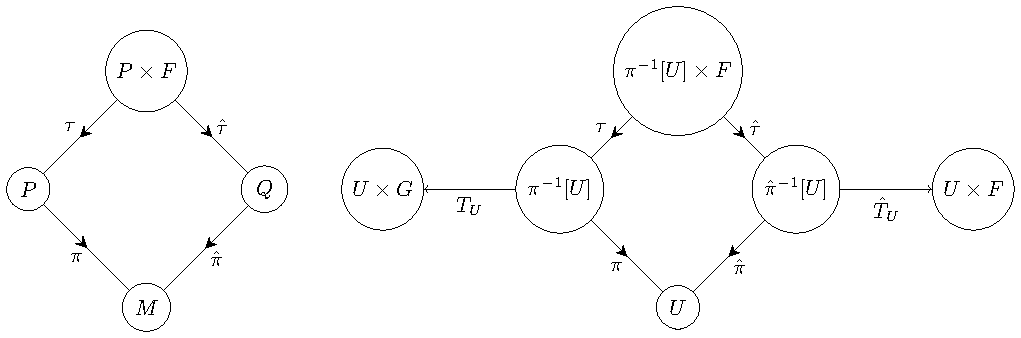
\includegraphics[width=0.9\textwidth]{../tikzpicture/I31.pdf}
  \caption{主丛和伴丛的映射}
  \label{fig:I-3-1}
\end{figure}

给定$P\times F \to M$两个渠道的映射,我们好奇两个方向的逆映射是怎样的,我们先来说明我们比较熟悉的方向$M\to P\to P\times F$,首先给定一点$x \in M$,那么$\pi^{-1}(x)$会将其映射为$p$ 点所在的fiber,而$\tau^{-1}$的逆映射应该作用到集合$\pi^{-1}(x)$上,
我们先来观察$\tau^{-1}$作用到$p$点的上给出 $(p,F)$这一子流形,所以$\tau^{-1}[\pi(x)]$最后的结果为\[
  \{(p, f)| f\in F, p \in \pi^{-1}(x)\} \equiv A
.\]
接下来我们说明另一个方向,我们同样考虑$x$点的逆映射,由于 $\hat{\pi}$ 是借助$\pi$来定义的,所以逆映射同样需要借用 $\pi^{-1}(x)$,我们考虑一点$p \in \pi^{-1}(x)$,由于没有限制$f \in F$所以对于借助$p$的 $\hat{\pi}$ 的逆映射$\hat{\pi}^{-1}$作用在$x$
点给出的集合为 \[
  \{p\cdot f \mid f \in F,\pi(p) = x\}
.\] 

\begin{figure}[htpb]
  \centering
  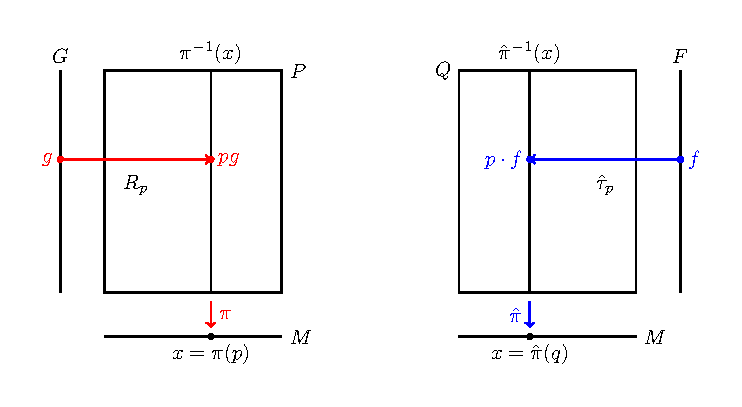
\includegraphics[width=0.8\textwidth]{../tikzpicture/I32.pdf}
  \caption{主丛和伴丛的对应}
  \label{fig:I-3-2}
\end{figure}
看图\ref{fig:I-3-2}可以精确理解该概念,和$p$点类似,同fiber的其它点也可以给出 $x$故最后给出 \[
  \hat{\pi}^{-1}(x) = \{ p \cdot f | f\in F,p \in \pi^{-1}(x)\} \equiv B
.\] 
随后,我们来看$\hat{\tau}^{-1}$,原则上应该作用于上面这个集合,也就是$\hat{\tau}^{-1}[B]$,我们希望两条路殊途同归,这里就需要满足$\hat{\tau}^{-1}[B] = A$.证明集合相等的方法我们已经熟悉,这里直接开始,对于$\forall b = p \cdot f \in B$,
根据定义 \ref{def:轨道}有 \[
\hat{\tau}^{-1}(b) = (p,f)g = (pg,g^{-1}f) \in  A,  \forall g\in G 
.\] 
故$B \subset A$,反过来对于$ \forall (p,f) \in A$\[
\hat{\tau}(p,f) = p \cdot f 
.\] 
由于两个集合的范围相同,故$a \in B$,则$A \subset  B$,故$A = B$,综合以上理解,对于点 $x$殊途同归,那么对于集合 $U \subset M$有\[
  \hat{\tau}^{-1}[\hat{\pi}^{-1}[U]] = \pi^{-1}[U] \times F
.\] 

在定义\ref{def:主纤维丛}定义主丛时要求是局域平凡,我们总可以找到$U\subset M$是平凡主丛,也就是图\ref{fig:I-3-1}右面所示,但是$\hat{T}_U$还没有定义,是否存在一个Q上的微分同胚映射$\hat{T}_U: \hat{\pi}^{-1}[U] \to U \times F$,
答案是存在,定义如下\[
  \hat{T}_U(q):= (\hat{\pi}(q),\breve{f}_U), \quad \forall q \in \hat{\pi}^{-1}[U] 
.\] 
其中$\breve{f}_U$ 满足$q = \breve{p}_U\cdot \breve{f}_U$(对于同一条轨道上,可以选择轨道上任一点代表这个轨道,而在一条轨道上,如果$p$固定, $f$便固定),而$\breve{p}_U$ 是$T_U$在纤维 $\pi^{-1}[\hat{\pi}(q)]$的特殊点,即$S_U(\breve{p}_U) = e$,当$\breve{p}_U$ 选定后,对于q点而言$\breve{f}_U$ 也就选中了.

接下来我们来说明$Q$是流形.前文说明了$Q$构成拓扑空间, 而$\hat{\pi}^{-1}[U]\subset Q$是开子集,开子集等证明借助$\hat{\pi}^{-1}[U]\times F$是$P\times F$给出,故结合上诱导拓扑则$\hat{\pi}^{-1}[U]$ 也构成拓扑空间.
\begin{note}
 设$(Q,\mathscr{Q})$是拓扑空间,$\mathscr{Q}$是$Q$的拓扑,而$U\subset Q$,所谓诱导拓扑就是给$U$定义一个拓扑 $\mathscr{U}$,使得$(U,\mathscr{U})\subset (Q,\mathscr{Q})$,$\mathscr{U}$定义为
 \[
   \mathscr{U}:=\{X \subset U \mid \exists Y \in \mathscr{Q}\quad s.t. X = U \cap Y\} 
 .\] 
 更详细内容见书P23.
\end{note}
根据流形的定义要求,我们只需要证明Q的任一开子集$\hat{\pi}^{-1}[U]$ 存在到$V_\alpha$($\mathbb{R}_n$ 中用通常拓扑衡量的开子集)的同胚映射,且两个开子集之间的交 同胚给出的 $V_\alpha$和 $V_\beta$ 之间的映射是$C^\infty$的.
直接证明比较困难,因为这是对 流形的要求,不过我们可以借助于其它流形诱导出的$V_\alpha$来给出$Q$是流形,也就是说只要证明$\hat{\pi}^{-1}[U]$同胚于某个流形,再对其它子集进行相同的操作便得到$Q$是流形.
我们在前文还没有证明$\hat{T}_U$ 是微分同胚,我们先证明其是同胚映射,并使得$Q$构成流形.证明是同胚映射要分两步走
 \begin{proof}
  \begin{enumerate}
    \item $\hat{T}_U$是一一到上的: 证明一一到上最简单也最直观的就是需要两个集合之间的元素一一对应,我们先列出需要证明的集合
      \begin{align*}
        \hat{\pi}^{-1}[U] &= \{q  \mid q = p \cdot f , p \in \pi^{-1}[U], f \in F\} \\
        U \times F & = \{(x,f)| x \in U, f \in F\}
      .\end{align*}
      由 $\hat{\pi}[\pi^{-1}[U]] = \pi[\pi^{-1}[U]]=U$,不难给出,坐标关于$x$的分量是一一对应的,接下来的问题只需要给出关于$f$的分量是一一对应的问题便解决了.我们只要证明 $\pi^{-1}(x), \forall x \in U$成立即可
      \begin{align*}
    \hat{\pi}^{-1}(x) = \{ p \cdot f(p) | p \in \pi^{-1}(x)\} = \{ \breve{p}_Ug \cdot f(\breve{p}_U g) | \forall g \in G\}
      .\end{align*}
      这里写成$f(p)$时因为对于固定 $q$点, $f$和 $p$的选择有关, 当 $g = e$时, $f(\breve{p}_Ug) = \breve{f}_U$,我们构造集合 \[
        \{\breve{p}_U \cdot g\breve{f}_U \mid \forall g \in G\} 
      .\] 根据定义\ref{def:左作用},可以给出上面集合和$F$微分同胚,我们知道 $p \cdot gf = p g\cdot f$,故上面关于$q$点的集合又可以写为\[
        \{\breve{p}_U g\cdot \breve{f}_U \mid \forall g \in G\} \equiv C
      .\] 
      ok,我们观察集合$\hat{\pi(x)^{-1}}(x)$ 和$C$,发现每有一个 $g \in G$,两个集合内都有一个点给出对应于$g$,且由于 $\hat{T}_U$关于$f$的映射,把$\hat{\pi}^{-1}(x)$ 的点映射为$C$上的点,也就说 $C$和 $\hat{\pi}^{-1}(x)$ 点点对应,即
      由$\hat{T}_U$ 一一到上成立.
      \begin{note}
       总结下思路,首先按开头的想法要证明两个集合之间的元素一一对应, 由于两个集合在映射$\hat{T}_U$关于$x$方向定义域相同,所以只要给出映射关于 $f$ 的分量一一对应即可,我们通过构造和$F$微分同胚的集合解决了问题.
      \end{note}
    \item 我们在证明一一到上时证明的是点点对应,故其满足连续定义所要求的拓扑结构,故正逆映射均为连续的.连续定义见P24定义3a.
  \end{enumerate} 
 \end{proof}
 \begin{note}
   介绍完数学方法后,我们还是来一些hand-waving,$Q$是流形的来源在于$Q$是一个高维度流形向低维度流形的投影,把 $(pg,g^{-1}f)$这一条轨道投影到一点,大的流形局部同胚与$\mathbb{R}^n$维,把轨道看作一点无非就是去掉
   李群 $G$作为流形时的维度,这里也暗示了 $Q$的维度是 $\dim{M}+ \dim{F}$,(在这里维度的表示只是一个直观的想法),所以 $Q$也可以看作是 $P\times F$的嵌入子流形.
 \end{note}
 随后$P\times F$是流形,其和嵌入子流形的关系是 $C^\infty$,原因是根据流形定义要求的第二点流行中相交的两个区域同胚于不同的 $\mathbb{R}^n$如果要求其中一个映射是恒等映射,另一个映射是 $\hat{T}_U$,那么其正逆映射均为$C^\infty$,最后$\hat{T}_U$ 是微分同胚映射.

 至此,我们可以说$Q$和 $P$十分相像,流形$Q$配 以上面要求后的数学结构称为\textbf{与主丛$\bm{P(M,G)}$相伴的纤维丛[fiber bundle associated to principal fiber bundle $\bm{P(M,G)}$]},简称为主丛$P$的伴丛,简记为 $(P\times F)/\sim  $.流形 $F$称为伴丛 $Q$的\textbf{典型纤维(typical fiber)}.
 最后还有一个问题就是关于转换函数的问题,我们根据$T_U$给出 $\hat{T}_U$,同样可以根据$T_V$给出 $\hat{T}_V$,其中$U\cap V \neq \varnothing$,根据定理\ref{thm:I-1-2}有 知道$\breve{p}$ 的转换关系,我们想问$\breve{f}$ 的关系是什么?
 \begin{align*}
   q = \breve{p}_U \cdot \breve{f}_U = \breve{p}_V \cdot \breve{f}_V =  \breve{p}_U g_{UV}(x) \cdot \breve{f}_V = \breve{p}_U \cdot g_{UV}(x) \breve{f}_V 
 .\end{align*}
故\[
  \breve{f}_U = g_{UV}(x) \breve{f}_V
.\] 
仿照局域截面还可以定义伴丛$Q$的局域截面,它是$C^\infty$映射$\hat{\sigma}: U\to Q$,满足\[
\hat{\pi}(\hat{\sigma}(x)) = x, \forall x \in U 
.\] 
伴丛的知识基本已经结束了,下面我们举一些例子来加深理解.
\begin{example}
 对任一主丛$P(M,G)$都可以看作是自己的伴丛. 
 \label{ex:I-3-1}
\end{example}
对主丛$P(M,G)$构造自己的伴丛,首先需要选定typical fiber  $F$,我们可以选择结构群 $G$作为$F$,随后应该定义结构群对typical fiber 的左作用 $\chi:G \times G(F) \to G(F)$,可以选择左平移为左作用,即\[
\chi_g(h) = gh, \forall g,h \in G 
.\] 
这样我们就可以得到伴丛$Q$,且有 \(q = p \cdot g, p \in  P, g \in G  \),我们可以很自然地定义映射$\nu : Q \to P$为\[
\nu(q) := pg \in P, \forall q = p\cdot g \in Q 
.\] 
从直观上看上面这个映射是微分同胚的,验证的话,首先一一到上性比较好验证,连续性根据定义也不困难,关键是怎么确定这个映射是$C^\infty$的,这个可以借助$P\times G(F)$是流形,就是图\ref{fig:I-3-1}左侧我们可以看到流形$P\times F$的存在开子集同胚于 $P $和$Q$,且由于$G = F$,在 $P\times G(F)$势必存在开子集的交包含 $P$和 $Q$,故交之间的映射是 $C^\infty$的,也就是$\nu$ 
是$C^\infty$,故$\nu$是微分同胚映射,也就是说 $P(M,G)$自身就是自己的伴丛.
\begin{example}
  \label{ex:I-3-2}
  我们在例\ref{ex:I-1-3}中定义了一个非平凡主丛,我们将其引过来并记作$S^1(S^1,Z_2)$.我们来看看如何定义这样非平凡主丛的伴丛.
\end{example}
令$F = \mathbb{R}$,则定义左作用 $\chi: Z_2 \times \mathbb{R} \to \mathbb{R}$为\[
  \chi_e(f) = \chi_h(f) := f, \forall f \in \mathbb{R}
.\] 另外对于$S^1 \times \mathbb{R}$有右作用 $\xi:(S^1 \times \mathbb{R}) \times G \to S^1 \times \mathbb{R}$为
\begin{align*}
  \xi_e(p_\theta,f)& = (p_\theta,f)\\
  \xi_h(p_\theta,f)& = (p_{\theta + \pi},f)
\end{align*}
右作用依赖于$P,F$上的作用,依照$P \times F$右作用可以给出$Q$的轨道,接下来我们来看看 $Q$,$Q$上每点对应的是集合 \[
  \left\{ (p_\theta,f),(p_{\theta + \pi},f) \right\} 
.\] 
故$Q$是这样一个流形, 其水平截面为 $S^1$,而竖直方向是流形 $F$,也就是说 $Q$微分同胚于 $S^1 \times F$,也就是说
 $Q$是整体平凡伴丛,可以给出微分同胚映射 \[
 \hat{T}_M(q):= (\pi(p_\theta),f), \quad \forall q = p_\theta\cdot f
 .\] 

 例子\ref{ex:I-3-2}给出平凡主丛最主要的原因是因为$F$上的左作用足够简单,简单到可以认为就是把流形 $F$在底流形
 的维度进行复制粘贴.我们可以推广到任意主丛上,对任一主丛,取 $F$为任意流形定义左作用为 $\chi:G \times F \to F$为
 \[
 \chi_g(f) := f , \quad \forall g \in G, f\in F
 .\]故可以给出$Q$为 \[
 q = \left\{ (pg,f) \mid  \forall g \in G \right\} \subset P\times F
 .\] 自然存在微分同胚映射\[
 \hat{T}_M=(pg,f)
 .\] 
 故以上步骤给出的伴丛是平凡伴丛.
 \begin{example}
   \label{ex:I-3-3}
   依旧选择例\ref{ex:I-1-3}的非平凡主丛$S^1(S^1,Z_2)$,仍取 $F = \mathbb{R}$,但左作用 $\chi:Z_2 \times \mathbb{R} \to \mathbb{R}$定义为\[
     \chi_e(f):= f, \chi_h(f) := -f , \forall f \in \mathbb{R}
   .\] 
 \end{example}
 我们来看这样的伴丛$Q$会发生什么样的变化,要给出伴丛,我们需要给出$\xi:\left( S^1 \times \mathbb{R} \right) \times Z_2 \to S^1 \times \mathbb{R}$来确定
 轨道,给出的左作用为
 \begin{align*}
   \xi_e(p_\theta,f) & = (p_\theta, f)\\
   \xi_h(p_\theta, f) & = (p_{\theta +\pi} , -f)
 .\end{align*}
 也就是说对于$Q$上一点 $q$实际上对应的是 \[
   \left\{ (p_\theta,f), (p_{\theta + \pi}, -f) \right\} 
 .\] 
 这对应于什么流形呢?我们再次回到例\ref{ex:I-3-2},不难发现例\ref{ex:I-3-2}无非就是一个圆柱面并且取了对径认同
 也就是说,对于圆柱面对着直径切开,拿其中一半再度接上,便是我们在例\ref{ex:I-3-2}所得的流形.而在本例无非就是沿
 直径切开后,取其中一半并把一个头翻转180度,并接上,就是我们所说的莫比乌斯环.结构如下图所示.
 \begin{figure}[htpb]
   \centering
   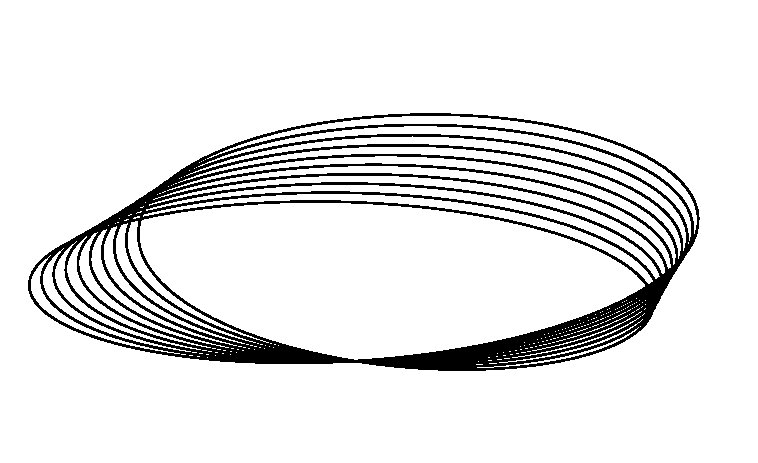
\includegraphics[width=0.6\textwidth]{../tikzpicture/I33.pdf}
   \caption{莫比乌斯环}
   \label{fig:I-3-3}
 \end{figure}
 \begin{note}
   还有一点值得说明的是,我第一次在书上看到按照\ref{ex:I-3-2}给出的是莫比乌斯环时是不太相信的,主要原因是因为莫比乌斯环在
   我的认知中是一个连续翻转的结构,但是例子中并没有强调这一点;实际上例\ref{ex:I-3-2}的定义更准确来说是定义了一个和莫比乌斯环
   同胚的结构.关于更详细了解莫比乌斯环的知识,这里有\href{https://www.bilibili.com/video/BV1u5NAefE9W}{视频}(点击跳转)
 \end{note}
 \begin{example}
   \label{ex:I-3-4}
   {\color{red}(切丛)} 维数是$n$的底流形 $M$的标架丛 $FM$的结构群 $G = GL(n)$借助合适的群作用可以给出 $FM$的伴丛是切丛.
 \end{example}
 取流形$F = \mathbb{R}^n$($\mathbb{R}^n$是矢量空间),则 $f = (f^1, \cdots ,f^n) \in F$,并定义左作用$\chi: G \times F \to F$为\[
   (\chi_g(f))^\mu := g^{\mu}{}_{\nu}f^\nu, \quad \forall g\in GL(n), f\in F 
 .\] 
 我们接下来就可以给出$FM$的伴丛 $Q$,首先需要右作用 $\xi:(FM \times F) \times G \to FM \times F$为\[
 \xi_g(p,f) =  \xi_g((x,e_\mu),f^\sigma) = ((x,e_\mu)g,g^{-1}(f^\rho)) = ((x,e_\nu g^{\nu}{}_{\mu} ),(g^{-1})^{\rho}{}_{\sigma}f^\sigma)
 .\]  
 接下来我们来看这样给出的伴丛为什么是切丛?给点$m_1 = ((x,e_\mu),f^\rho) \in FM \times F$可以构造一个矢量\[
   v_a = (e_\mu)_a f^\mu \in T_xM 
 .\] 
 如果给另一个点$m_2=((x,e'_\mu),f'^\rho) \in FM \times F$,$m_1$和 $m_2$对应于底流形上同一个点 $x$,同样可以构造$m_2$点的矢量 \[
   v'_a = (e'_\mu) f'^\mu \in T_xM 
 .\] 
 如果$m_1$和 $m_2$同轨道的话,它们之间满足关系 $m_2 = m_1g$,即 \[
 m_2 = m_1g = ((x,e_\nu g^{\nu}{}_{\mu}),(g^{-1})^{\rho}{}_{\sigma}f^\sigma)
 .\] 
 故\[
   v'_a = (e_\nu)_a g^{\nu}{}_{\mu} (g^{-1})^{\mu}{}_{\sigma}f^\sigma = (e_\nu)_a \delta^{\nu}{}_{\sigma}f^\sigma = (e_\nu)_a f^\nu = (e_\mu)_a f^\mu = v_a
 .\] 
 也就说同轨道的点给出$T_xM$上的同一个矢量.这就表明 $\hat{\pi}^{-1}[x]$ 和$T_xM$存在一一对应关系,于是
  $Q$可以看作 $M$的切丛 $TM$.此时伴丛 $Q$的局域截面,对应于 $M$上的一个矢量场.
  \begin{example}
    \label{ex:I-3-5}
  {\color{red}(余切丛)}有了切丛,我们就可以定义余切丛,本例来看如何定义余切丛.
  \end{example}
  仍然取$P = FM$,$G = GL(n)$, $F = (\mathbb{R}^n)^* = \mathscr{T}_{\mathbb{R}^n}(0,1)$,则$f \in F$是$\mathbb{R}^n$上的对偶矢量,记作 $(f_1,\cdots,f_n)$,定义$\chi:G \times F \to F$为
  \begin{equation}
    (\chi_g(f))_\mu := (g^{-1})^{\nu}{}_{\mu}f_\nu, \quad \forall g \in GL(n), f \in F 
    \label{eq:I-3-1}
  \end{equation}
  这个作用我们暂且先接受,为何这么定义后续讨论.给定点$((x,e_\mu), f_\rho) \in FM \times F$可以构造$x \in M$的对偶矢量\[
  \beta \equiv e^\mu f_\mu \in T^*_xM, 
.\] $\{e^\mu\}$是 $\{e_\mu\}$的对偶基底.接下来的思路只要证明同轨道的点对应于同一个对偶矢量,就可以
给出此时的 $Q$时余切丛,开始之前,我们应该来看为什么 $F$上的左作用按照式\ref{eq:I-3-1}定义,对于对偶矢量
我们有 \[
  \beta_a = (e^\mu)_a f_\mu
.\] 
对偶基矢作用于基矢上有作用\[
  e^\mu e_\mu = C ,\quad C\in\mathbb{R} 
.\]
当基矢量发生线性变换$e'_\rho = e_\mu g^{\mu}{}_{\rho} $后,我们需要重新求得对偶基矢满足上式且$C$不变给出\[
  e_\mu g^{\mu}{}_{\rho} (g^{-1})^{\rho}{}_{\mu} e^\mu = C 
.\] 
不难得出\[
e'^\rho = (g^{-1})^{\rho}{}_{\mu}e^\mu
.\] 
随后我们给出关于$f_\mu$的变化 \[
f'_\mu = g^{\nu}{}_{\mu}f_\nu
.\] 
事情到这里发现这里和\ref{eq:I-3-1}差了一个逆,是不是我们哪里有算错,仔细检查后发现没有算错,那问题出现在了哪里;
实际上,问题出现在了$\xi_g = (R_g(p),\chi_{g^{-1}}(f))$ 上,仔细观察发现$\chi_g$和 $g$作用到 $f_\mu$上正好差了一个逆.
最后,我们给出 式\ref{eq:I-3-1}要求的左作用.我们通过坐标变换给出的左作用,接下来我们验证一下同轨道的点给出相同的对偶矢量.
还是给出$m_1 = ((x,e_\mu), f_\rho)$,这时构造的对偶矢量为\[
\beta_a = (e^\mu)_a f_\mu
.\]
另取一点$m_2 = m_1g = ((x,e_\mu g^{\mu}{}_{\nu}),g^{\rho}{}_{\sigma}f_\rho)$,此时给出的为 \[
\beta'_a = (g^{-1})^{\nu}{}_{\mu}(e^\mu)_a g^{\rho}{}_{\nu}f_\rho = (e^\mu)_a f_\rho = \beta_a
.\] 
故同轨道的点给出的是$T^*_xM$的矢量.最后我们给出了主丛的伴丛为余切丛的构造方法.局域截面是对偶矢量场.
 \begin{note}
  这里的主丛取得是标架丛,每个标架对应于一个对偶标架,故标架丛同胚于对偶标架丛$FM^*$,我们可以给出$\xi_g:(FM^* \times F) \times G \to FM^* \times F$
  使得上面定义有更自然的结构.\[
    \xi_g(p,f) = \xi_g((x,e^\mu),f_\sigma) = ((x,(g^{-1})^{\mu}{}_{\nu}e^\nu),g_{\rho}{}^{\sigma}f_\sigma)
  .\] 
\end{note}
\begin{example}
  \label{ex:I-3-6}
  {\color{red}(1,1)型张量丛} 仍然以标架丛$FM$为主丛,我们来看如何给出张量丛.
\end{example}
首先还应该选择$F$,此时 $F$应该为 $\mathbb{R}^n$上(1,1)型张量,$f^{\mu}{}_{\nu}$ 代表在坐标基上的分量,随后我们定义
左作用,参考例\ref{ex:I-3-4}和例\ref{ex:I-3-5}给出$\chi:G\times F \to F$为\[
  (\chi_g(f))^{\mu}{}_{\nu} := g^{\mu}{}_{\alpha}(g^{-1})^{\beta}{}_{\nu}f^{\alpha}{}_{\beta} \quad\forall g\in GL(n), f\in F 
.\] 
现在每点$((x,e_\mu),f^{\rho}{}_{\sigma})\in FM \times F$自然给出$x\in M$上的一个(1,1)型张量为\[
T^{a}{}_{b} \equiv f^{\mu}{}_{\nu}(e_\mu)^a(e^\nu)_b
.\] 
和前面两个例子一样的道理,如果$P\times F$上的点同轨道,那么就应该对应于同一个张量,故此时的伴丛是(1,1)型张量丛.局域截面是(1,1)型张量丛.

例\ref{ex:I-3-4},例\ref{ex:I-3-5}和\ref{ex:I-3-6}给出的是一样的例子,由此可以推广至$(k,l)$型张量丛的构造.我们重新回顾如何构造伴丛的,给定主丛$P(M,G)$,
然后我们选择不同的 $F$,并在 $F$上定义左作用.根据定义\ref{def:李变换群}不难发现$\hat{G}\equiv\{\chi_g : F\to F \mid g\in G\}$是李变换群.根据定义\ref{def:实现}
的表述,可以给出$F$是 $G$的实现空间.根据定义\ref{def:表示和表示空间和忠实表示}当 $F$是矢量空间且$\chi_g:F\to F$是线性变换时,此时$\hat{G}$ 是一个表示,$F$
是表示空间,此时得到的伴丛 $Q$称为\textbf{伴矢丛(associated vector bundle)},也简称为\textbf{矢丛}.切丛,余切丛和(k,l)张量丛都是矢丛.

由于$F$是矢量空间,由图\ref{fig:I-3-2},我们知道存在同胚映射$\hat{\tau}_p$ 使得$\hat{\pi}^{-1}(x)$ 也是一个矢量空间,我们可以借助$F$上的矢量加法和数乘定义出
$\hat{\pi}^{-1}(x)$ 的加法和数乘为\[
  q_1\pm q_2 := p\cdot(f_1 \pm f_2), \quad \alpha q_1 := p \cdot \alpha f_1, \forall \alpha \in \mathbb{R}(\mathbb{C}) 
.\] 
零元定义为\[
0 : = p\cdot 0
.\] 
上面定义目前看来比较合理,但还是存在一些问题,我们知道$Q$上的点是 $P\times F$上的一条轨道,我们可以选取轨道上的任一点代表 $q$点,上面选择了 $p\cdot f$,
我们同样可以选择$p' \cdot f'$,那么重复上面的定义给出的两套规则是否相同?这是需要我们证明的,我们有
\begin{align*}
  p' \cdot (f_1' \pm f_2')&= pg \cdot (g^{-1}f_1 \pm g^{-1}f_2)\\
                          &= pg \cdot(\chi_{g^{-1}}f_1 \pm \chi_{g^{-1}}f_2)\\
                          & = pg \cdot \chi_{g^{-1}}(f_1 \pm f_2)\quad \chi_g\text{是线性的}\\
                          & = pg \cdot g^{-1}(f_1 \pm f_2)\\
                          & = p gg^{-1} \cdot (f_1 \pm f_2)\\
                          & = p \cdot (f_1 \pm f_2) 
.\end{align*}
数乘和零元也可按照上面方法验证.也就是说$\hat{\pi}^{-1}(x)$ 是一个矢量空间,这也是我们简称为矢丛的原因.每个矢量空间都有零元,也就是说不管平凡与否,
任意矢丛都有一个整体截面$\hat{\sigma}$,满足$\hat{\sigma}(x) = 0 \in \hat{\pi}^{-1}(x)\quad \forall x\in M$,称为\textbf{零截面}.
\end{document}
